\documentclass[11pt]{article}

% =====================================================================
%  SCUDEM XI 2026, Problem A --- final report
%  Compile with pdfLaTeX (e.g. Overleaf). Needs the folder figures/ next to
%  this file with the 11 PNGs it includes (growth_fits, arm_headline,
%  arm_tornado, arm_growth_spurt, first_pass_km_vs_model,
%  first_pass_competing_risks, first_pass_rho_sweep, final_bootstrap_constants,
%  final_fit, final_arm_prediction, final_arm_sobol).
%  Figures are made by figures/make_figures.m, figures/arm_sensitivity.m,
%  rmse_first_pass/*.m (first pass) and final_study/scripts/overnight_rmse.m
%  (final; the final_* figures are copies of final_study/results/full/fig_*.png).
%  Build the Overleaf zip with:  python build_overleaf_zip.py
% =====================================================================

% ---------- packages ----------
\usepackage[T1]{fontenc}
\usepackage[a4paper,margin=2cm]{geometry}
\usepackage{lmodern}
\usepackage{microtype}
\usepackage{amsmath,amssymb,amsthm}
\usepackage{booktabs}
\usepackage{array}
\usepackage{longtable}
\usepackage{multirow}
\usepackage{enumitem}
\usepackage{xcolor}
\usepackage{graphicx}
\usepackage[font=small,labelfont=bf]{caption}
\usepackage{tikz}
\usetikzlibrary{arrows.meta,angles,quotes,calc,positioning}
\PassOptionsToPackage{hyphens}{url}
\usepackage[colorlinks=true,linkcolor=blue!60!black,citecolor=blue!60!black,urlcolor=blue!60!black]{hyperref}

\graphicspath{{figures/}}

% ---------- team details (edit before submission) ----------
\newcommand{\teamname}{SCUDEM XI 2026 Team}

% ---------- convenience macros ----------
\newcommand{\dd}[2]{\frac{d #1}{d #2}}
\newcommand{\pd}[2]{\frac{\partial #1}{\partial #2}}
\newcommand{\eps}{\varepsilon}
\newcommand{\lift}{u_{\mathrm{lift}}}
\newcommand{\lfa}{\ell_{\mathrm{fa}}}
\newcommand{\lua}{\ell_{\mathrm{ua}}}
\newcommand{\Fax}{F_{\mathrm{ax}}}
\newcommand{\tgt}{\mathrm{tgt}}
\newcommand{\pluspart}[1]{\left\langle #1 \right\rangle_{+}}
\newcolumntype{L}[1]{>{\raggedright\arraybackslash}p{#1}}

\theoremstyle{definition}
\newtheorem{remark}{Remark}
\newtheorem{proposition}{Proposition}

\title{\textbf{A Growth--Statics Model for Paediatric Prosthetic Socket Replacement}\\[4pt]
\large SCUDEM XI 2026, Problem A}
\author{\teamname}
\date{November 2026}

\begin{document}
\maketitle

\begin{abstract}
We build a mathematical model that predicts \emph{whether, and at what age}, a child's transradial (below-elbow) prosthetic socket reaches a point of substantial change that warrants adjustment or replacement as the residual limb grows. The model has four layers: (i) a \textbf{logistic growth ordinary differential equation} (ODE) for residual-limb length and circumference, fitted to the anthropometry of 3,900 children; (ii) a \textbf{socket-fit map} that turns the growth trajectory into tightness and distal-clearance signals; (iii) a \textbf{planar lift statics} block for a set of actions (a hold and a curl, plus a straight-arm reach for an optional shoulder-load extension), whose axial load feeds back onto the clearance criterion; and (iv) a closed-form \textbf{threshold} rule that combines three criteria --- tightness, distal clearance with pistoning, and prosthetic length discrepancy --- into the time to intervention $T^*$. Because paediatric casefiles exist only for the leg, we \textbf{validate on the leg and predict on the arm}. We use raw casefiles of 59 Cambodian children, with per-socket fitting ages, and individual growth records of 3,900 children. Calibrated on 188 transtibial socket episodes, the model reproduces their Kaplan--Meier curve with RMSE $0.015$ ($R^2=0.997$), and the same holds when each child is left out in turn (RMSE $0.015$). It predicts 85 held-out knee-disarticulation and transfemoral episodes with RMSE $0.023$ ($R^2=0.992$). All of these errors lie below the sampling noise of the data, and the model clearly beats exponential and Weibull fits. A competing-risks version also reproduces \emph{which} problem occurs: in the leg, most problems coded ``tight'' are the limb reaching the end of the socket. All calibrated constants carry 95\% confidence intervals from 5,250 child-level bootstrap refits and lie within clinical ranges. For the arm, the median child fitted between ages 4 and 10 needs intervention after 10--12 months (boys) or 11--16 months (girls), and one child in ten lasts roughly two years or more. These intervals agree with the clinical guidance that a child's upper-limb fit be revised annually, and translate into a simple schedule: review about 8 months after fitting for children fitted before age 8. Distal clearance, not tightness, is the binding criterion; the arm's length tolerance and built-in clearance are the inputs that most change the answer. The load lifted matters little: everyday objects bring the threshold forward by about one month.
\end{abstract}

\vspace{4pt}
\noindent\fbox{\begin{minipage}{0.97\textwidth}
\textbf{Results at a glance}
\begin{itemize}[leftmargin=1.4em,itemsep=1pt,topsep=3pt]
\item \textbf{Growth:} the logistic ODE fits every limb measurement within $0.32$--$0.89$\,cm (at most $2.9\%$ of adult size) across ages 2--18 (Table~\ref{tab:fits}).
\item \textbf{Validation (leg, final):} RMSE $0.0150$ on calibration, $0.0152$ leaving each child out, and $0.0228$ on held-out amputation levels, all below the child-level noise floor of $0.033$. For comparison, an exponential fit scores $0.060$ and a Weibull fit $0.035$ (Tables~\ref{tab:finalmetrics}, \ref{tab:bench}).
\item \textbf{Final constants} (95\% CI, 5,250 child-level refits): clearance $\delta_0/\rho=1.60$\,cm (1.16--3.04), leg length tolerance $2.26$\,cm (1.50--4.51), spread $\sigma=0.63$ (0.43--0.96), tightness tolerance $\Gamma\gtrsim0.15$. All lie within clinical ranges (Table~\ref{tab:final}).
\item \textbf{Which problem:} in the leg, first problems are 65\% distal clearance, 34\% length and 1\% tightness. This reproduces the observed tight/short split (RMSE $\le0.014$) and matches prosthetists heating out the distal end of the socket most (Section~\ref{sec:final}).
\item \textbf{Prediction (arm):} for fitting ages 4--10, the median child needs intervention after $10$--$12$ months (boys) or $11$--$16$ months (girls), with 95\% CIs reaching roughly 3--6 months either side; the interval lengthens after puberty (Table~\ref{tab:arm}, Figure~\ref{fig:armfinal}).
\item \textbf{What matters:} the arm length tolerance (75\% of variance) and the clearance built into the socket (34\%). The lifted load moves $T^*$ by about 1 month, because children's objects piston the socket by about 1\,mm at most (Section~\ref{sec:sobol}).
\item \textbf{Limits:} the arm values of $\delta_0$, $\rho$ and $\Delta L_{\max}$ are unmeasured. The model predicts populations of sockets well but individual children only weakly (C-index 0.58). The pubertal spurt moves $T^*$ by up to 9 months. $R^2=0.9999$ is not attainable with 188 episodes (Section~\ref{sec:r2}).
\end{itemize}
\end{minipage}}

\tableofcontents

% =====================================================================
\section{Problem and approach}
\label{sec:intro}
% =====================================================================
A child's residual limb keeps growing after a prosthesis is fitted; the socket does not. Growth therefore drives the two universal problems reported by paediatric prosthetists: the socket becomes \emph{tight}, and the prosthesis becomes \emph{short} relative to the intact limb \cite{ghidini2025}. Clinically, socket adjustments occur on average every $8.3\pm6.6$ months and full replacements every $16.4\pm9.9$ months in Cambodian casefiles \cite{ghidini2025}. We ask when, for a child fitted with a below-elbow socket at age $a_0$, growth produces a \emph{substantial change} that requires intervention, and how that answer depends on the socket design and on the loads the child lifts.

Our approach chains four layers (Figure~\ref{fig:pipeline}). Every layer is solved in closed form, so the headline quantity $T^*(a_0)$ is an explicit formula whose sensitivity to each input can be differentiated directly. All constants are either fitted to data, taken from the literature, or calibrated against clinical outcomes; Section~\ref{sec:vars} lists every one with its value and source.

\begin{figure}[htbp]
\centering
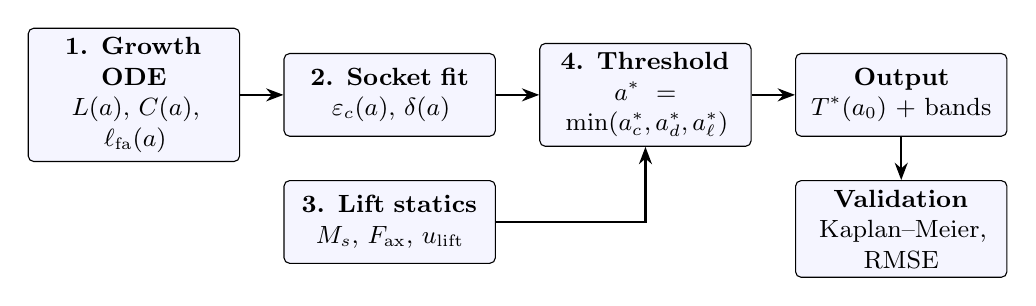
\begin{tikzpicture}[
  box/.style={draw,rounded corners=2pt,align=center,minimum height=1.05cm,text width=2.45cm,font=\small,fill=blue!4},
  arr/.style={-{Stealth[length=2.2mm]},thick}]
\node[box] (g) {\textbf{1. Growth ODE}\\ $L(a)$, $C(a)$, $\lfa(a)$};
\node[box,right=0.55cm of g] (s) {\textbf{2. Socket fit}\\ $\eps_c(a)$, $\delta(a)$};
\node[box,right=0.55cm of s] (t) {\textbf{4. Threshold}\\ $a^*=\min(a^*_c,a^*_d,a^*_\ell)$};
\node[box,right=0.55cm of t] (o) {\textbf{Output}\\ $T^*(a_0)$ + bands};
\node[box,below=0.55cm of s] (l) {\textbf{3. Lift statics}\\ $M_s$, $\Fax$, $\lift$};
\node[box,below=0.55cm of o] (v) {\textbf{Validation}\\ Kaplan--Meier, RMSE};
\draw[arr] (g) -- (s); \draw[arr] (s) -- (t); \draw[arr] (t) -- (o);
\draw[arr] (l) -| (t); \draw[arr] (o) -- (v);
\end{tikzpicture}
\caption{Model pipeline. Data enter at layer 1 (Snyder anthropometry) and at the validation step (Ghidini casefiles).}
\label{fig:pipeline}
\end{figure}

\subsection{Assumptions}
\label{sec:assumptions}
\begin{enumerate}[label=\textbf{A\arabic*.},ref=A\arabic*,leftmargin=2.6em,itemsep=1pt]
\item \label{as:logistic} Limb length and circumference follow logistic growth toward an adult size; the pubertal spurt is not modelled separately (Remark~\ref{rem:spurt}).
\item \label{as:rho} Residual-limb length is a fixed fraction $\rho$ of intact length; residual circumference grows like the intact limb's.
\item \label{as:snyder} Growth curves of US children measured in the 1970s \cite{snyder1977} represent the growth of the children in question; residual and population differences enter only through $\rho$ and the tolerances.
\item \label{as:socket} The socket is rigid, built once at $a_0$ with oversize $s_C$ and distal clearance $\delta_0$, and is not adjusted before the first threshold is reached.
\item \label{as:transfer} Only dimensionless tolerances (here $\Gamma$) transfer from leg to arm; dimensional ones ($\delta_0/\rho$, $\Delta L_{\max}$) do not.
\item \label{as:statics} Lifting is quasi-static and planar; the forearm, socket and prosthesis form one rigid segment; the liner acts as a linear axial spring.
\item \label{as:trigger} An intervention is needed as soon as any one criterion reaches its tolerance.
\end{enumerate}

% =====================================================================
\section{Variables, constants and their values}
\label{sec:vars}
% =====================================================================
Table~\ref{tab:vars} lists every quantity in the model. \emph{Type}: S = state (solved by the ODE); P = parameter (fitted, from literature, or calibrated); I = input (chosen or swept); D = derived; O = output or observed. Values marked \emph{arm} are used for the prediction (Section~\ref{sec:headline}); values marked \emph{leg} are used for validation (Section~\ref{sec:validation}). Lengths are in cm except moment arms, which are in m so that moments are in N\,m. M = boys, F = girls.

{\footnotesize
\renewcommand{\arraystretch}{1.18}
\setlength{\tabcolsep}{3pt}
\begin{longtable}{@{}L{1.55cm}L{4.25cm}L{1.05cm}L{1.0cm}L{5.3cm}L{2.2cm}@{}}
\caption{All variables and constants, with the values used.}\label{tab:vars}\\
\toprule
Symbol & Meaning & Unit & Type & Value used & Source\\
\midrule
\endfirsthead
\multicolumn{6}{@{}l}{\small\emph{Table~\ref{tab:vars} continued}}\\
\toprule
Symbol & Meaning & Unit & Type & Value used & Source\\
\midrule
\endhead
\midrule
\multicolumn{6}{r@{}}{\small\emph{continued on next page}}\\
\endfoot
\bottomrule
\endlastfoot
\multicolumn{6}{@{}l}{\textbf{Layer 1: growth}}\\
$a$ & age (independent variable) & yr & -- & data 2--18; predictions for 3--17 & --\\
$a_0$ & age when the socket is fitted & yr & I & swept 3--17. Validation (final): age at amputation + delay + years since first visit, per episode (196 of 273); others imputed & \cite{ghidiniData}\\
delay & years from amputation to first clinic visit & yr & P & \textbf{0.0001} (95\% CI 0.0000--0.0002): fitted soon after amputation & Sec.~\ref{sec:final}\\
$p_{\mathrm{boy}}$ & share of boys by amputation level & -- & D & TT 0.62, KD 0.83, TF 0.86 & \cite{ghidiniData}\\
$\lfa(a)$ & intact forearm length (radiale--stylion) & cm & S & logistic with $K_\Lambda, r_\Lambda, a_{50}$ & \cite{snyder1977}\\
$K_\Lambda$ & adult intact forearm length & cm & P & M 29.67, F 25.82 (at the 10\% cap) & fit to \cite{anthrokids}\\
$r_\Lambda$ & forearm length growth rate & yr$^{-1}$ & P & M $0.156\pm0.004$, F $0.166\pm0.007$ & fit\\
$a_{50}$ & age at half adult size (each curve) & yr & P & forearm length M 4.15, F 2.68; forearm circ.\ M 3.56, F 0.07; shank M 4.67, F 3.38; calf M 3.63, F 2.15 & fit\\
$a_b$ & baseline age of the closed form & yr & I & $a_b=a_{50}$, so that $B=1$ & --\\
$B_L,B_C,B_\Lambda$ & logistic constants $(K-y_b)/y_b$ & -- & D & $1$ when $a_b=a_{50}$; in general $e^{\,r(a_{50}-a_b)}$ & eq.~\eqref{eq:a50}\\
$\rho$ & residual-to-intact length ratio & -- & P & \emph{arm}: 1 (earliest, conservative), band 0.5--1. \emph{leg}: not identifiable on its own; only $\delta_0/\rho$ is (final 1.60\,cm) & Secs.~\ref{sec:sweep}, \ref{sec:final}\\
$L(a)$ & residual limb length, $\rho\,\lfa(a)$ & cm & S & logistic & eq.~\eqref{eq:rho}\\
$K_L$, $r_L$ & adult residual length; its growth rate & cm, yr$^{-1}$ & D & $K_L=\rho K_\Lambda$, $r_L=r_\Lambda$ & eq.~\eqref{eq:rho}\\
$C(a)$ & residual limb circumference & cm & S & logistic with $K_C, r_C, a_{50}$ & Assum.~\ref{as:rho}\\
$K_C$ & adult forearm circumference & cm & P & M 31.01, F 25.57 (at the cap) & fit to \cite{anthrokids}\\
$r_C$ & circumference growth rate & yr$^{-1}$ & P & M $0.108\pm0.002$, F $0.125\pm0.003$ & fit\\
$K^{\mathrm{leg}}_\Lambda, r^{\mathrm{leg}}_\Lambda$ & intact shank length: adult size, rate & cm, yr$^{-1}$ & P & M 42.92, 0.184; F 38.41, 0.212 & fit\\
$K^{\mathrm{leg}}_C, r^{\mathrm{leg}}_C$ & calf circumference: adult size, rate & cm, yr$^{-1}$ & P & M 41.11, 0.126; F 37.30, 0.143 & fit\\
$K_1,r_1,a_1,K_2,r_2,a_2$ & two-phase (bi-logistic) growth constants, used to test the spurt & cm, yr$^{-1}$, yr & P & spurt centre $a_2$: forearm length M 13.6, F 10.3; circumference M 14.8, F 10.4; full values in Table~\ref{tab:spurt} & fit to \cite{anthrokids}\\
$M_b(a)$ & body mass & kg & D & Snyder means; age 4: M 17.6, F 17.2; 10: M 35.4, F 35.1; 16: M 67.3, F 56.3 & \cite{snyder1977}\\
$\lua(a)$ & upper-arm length & m & D & age 4: M 0.214, F 0.211; 10: 0.292, 0.292; 16: 0.368, 0.338 & \cite{snyder1977}\\
\midrule
\multicolumn{6}{@{}l}{\textbf{Layer 2: socket fit}}\\
$s_C$ & intentional circumferential oversize & -- & I & $\approx0.04$--$0.06$ (2--3 sock layers, each $\approx2\%$ of circumference) & \cite{ghidini2025,sockply}\\
$\eps_{\max}$ & tolerable tightness & -- & P & literature $\approx0.025$; implied by the final $\Gamma\gtrsim0.15$: at least 0.08--0.10 & \cite{patent,volume1}\\
$\Gamma$ & combined tolerance $(1+s_C)(1+\eps_{\max})-1$ & -- & P & \textbf{final 0.255} (95\% CI 0.147--0.260; only bounded below, $\Gamma\gtrsim0.15$); first pass 0.121; literature 0.005--0.26 & Tab.~\ref{tab:final}\\
$\delta_0$ & initial distal clearance & cm & I & 0.5--3 in clinic; \emph{arm}: 1.5 (band 1--3) & \cite{ghidini2025}\\
$C_s$, $D_s$ & socket circumference; socket depth & cm & D & $(1+s_C)C(a_0)$; $L(a_0)+\delta_0$ & eq.~\eqref{eq:socket}\\
$\eps_c(a)$ & tightness $(C-C_s)/C_s$ & -- & D & starts at $-s_C/(1+s_C)$ & eq.~\eqref{eq:epsc}\\
$\delta(a)$ & distal clearance $D_s-L(a)$ & cm & D & starts at $\delta_0$ & eq.~\eqref{eq:delta}\\
\midrule
\multicolumn{6}{@{}l}{\textbf{Layer 3: lift statics}}\\
$g$ & gravitational acceleration & m\,s$^{-2}$ & -- & 9.81 & standard\\
$m_p$ & prosthesis mass & kg & I & 0.13--0.24; \emph{arm} central 0.24 & \cite{frontiers2022,dukecase}\\
$m_o$ & lifted object mass & kg & I & 0.165 / 0.33 / 0.66; central 0.33 & \cite{luciw2014}\\
$\ell_h$ & elbow to hand, fixed at $a_0$ & m & D & Snyder elbow--hand length; age 4: M 0.280, F 0.275; 10: 0.375, 0.374; 16: 0.474, 0.428 & \cite{snyder1977}\\
$\ell_p$ & elbow to prosthesis centre of mass, fixed at $a_0$ & m & I & assumed $0.5\,\ell_h$ (swept 0.4--0.7\,$\ell_h$); does not affect $T^*$ & assumption\\
$\varphi$ & forearm angle from the downward vertical & deg & I & hold A: 90; curl B: 150; reach C: 90 & --\\
$M_s$ & socket bending moment & N\,m & D & age 10 (M): hold 1.66, curl 0.83; ages 4--16: 1.24--2.09 (hold) & eq.~\eqref{eq:lift}\\
$\Fax$ & axial socket load ($+$ pull-off, $-$ push-on) & N & D & hold 0; curl $-4.84$ (central masses), range $-2.5$ to $-7.7$ & eq.~\eqref{eq:lift}\\
$k_s$ & liner and soft-tissue axial stiffness & N\,cm$^{-1}$ & P & $\approx75$ (adult transtibial; $\approx4$\,mm per 30\,N) & \cite{gholizadeh2011}\\
$\lift$ & curl pistoning displacement $|\Fax|/k_s$ & cm & D & 0.065 central; 0.033--0.102 over the mass ranges & eq.~\eqref{eq:ulift}\\
\midrule
\multicolumn{6}{@{}l}{\textbf{Layer 4: threshold}}\\
$\Delta L(a)$ & prosthetic length discrepancy $\lfa(a)-\lfa(a_0)$ & cm & D & -- & eq.~\eqref{eq:aell}\\
$\Delta L_{\max}$ & tolerable length discrepancy & cm & P & \emph{leg}, \textbf{final 2.26} mean child (95\% CI 1.50--4.51), 1.85 median child; clinic $\approx1$ fixable, up to 2 seen. \emph{arm}: assumed 2 (range 1--3) & Tab.~\ref{tab:final}, \cite{ghidini2025,ghidiniPoster}\\
$\delta_0/\rho$ (leg) & intact growth that closes the leg clearance & cm & P & \textbf{final 1.60} mean child (95\% CI 1.16--3.04), 1.31 median child & Tab.~\ref{tab:final}\\
$\lambda$ & leg length-type threshold $\min(\delta_0/\rho,\Delta L_{\max})$ & cm & P & first pass only: 1.95 (1.1--1.95 across stand-ins); literature 0.5--2. Replaced in the final fit by separate $\delta_0/\rho$ and $\Delta L_{\max}$ & Sec.~\ref{sec:calib}\\
$\sigma$ & child-to-child spread of the tolerances (log-SD) & -- & P & \textbf{final 0.63} (95\% CI 0.43--0.96); first pass 0.77 & Tab.~\ref{tab:final}\\
$C_\tgt,\,L_\tgt,\,\Lambda_\tgt$ & targets at which each criterion fires & cm & D & eqs.~\eqref{eq:Ctgt}, \eqref{eq:Ltgt}, \eqref{eq:Lamtgt} & --\\
$a^*_c,a^*_d,a^*_\ell$ & tightness, clearance, length ages & yr & O & closed form; $+\infty$ if the target is never reached & eqs.~\eqref{eq:acsol}--\eqref{eq:aellsol}\\
$a^*$, $T^*$ & threshold age; time to intervention & yr, mo & O & \emph{arm}, $a_0=4$--16: median child 9.8--22.6 (M), 10.7--35.4 (F), with 95\% CIs; mean-tolerance child 14.9--38.0 (M), 16.5--64.2 (F) & Table~\ref{tab:arm}\\
$a_{0,c}^{\max}$ & latest fitting age at which tightness can still fire & yr & D & $a_{50}-\ln\Gamma/r_C$ at $\Gamma=0.255$: M 16.2, F 11.0 & eq.~\eqref{eq:cutoff}\\
\midrule
\multicolumn{6}{@{}l}{\textbf{Validation}}\\
$T_{\mathrm{obs}}$, $e$ & observed months to first growth problem; event flag & mo, -- & O & 273 episodes (TT 188, KD 20, TF 65), 155 events & \cite{ghidiniData}\\
$\widehat S(t)$ & Kaplan--Meier survivor estimate & -- & O & TT median 11.8 months; 48\% problem-free at 12 months & eq.~\eqref{eq:km}\\
RMSE, $R^2$ & model vs.\ Kaplan--Meier, monthly grid & -- & O & \textbf{final}: TT 0.0150 / 0.997; leave-one-child-out 0.0152 / 0.997; KD+TF 0.0228 / 0.992; noise floor 0.033; Weibull 0.035 / 0.983 & Tables~\ref{tab:finalmetrics}, \ref{tab:bench}\\
$F_{\mathrm{tight}},F_{\mathrm{short}}$ & cumulative incidence of tight / short problems & -- & O & TT at 25 months: 0.54 / 0.27; final model RMSE 0.014 / 0.008 & Tab.~\ref{tab:finalmetrics}\\
C, IBS & concordance; integrated Brier score & -- & O & TT: C 0.58, IBS 0.187 (null 0.177); KD+TF: C 0.64, IBS 0.160 (null 0.166) & Tab.~\ref{tab:finalmetrics}\\
\midrule
\multicolumn{6}{@{}l}{\textbf{Extension: shoulder load}}\\
$\tau_{\mathrm{sh}}(a)$ & shoulder torque in the reach & N\,m & D & age 4: 2.43; 10: 3.29; 16: 4.15 (M, central masses) & eq.~\eqref{eq:shoulder}\\
$S(a)$ & strength proxy $\propto M_b^{2/3}$ & -- & D & relative & eq.~\eqref{eq:shoulder}\\
$\tau_{\mathrm{sh}}/M_b^{2/3}$ & shoulder load index & N\,m\,kg$^{-2/3}$ & O & 0.360 (age 4) falling to 0.251 (age 16) & Sec.~\ref{sec:ext}\\
\end{longtable}
}

% =====================================================================
\section{Layer 1 --- the growth ODE}
\label{sec:growth}
% =====================================================================

\subsection{Model statement}
We treat residual-limb length $L$ and circumference $C$ as logistic growth processes decelerating toward adult asymptotes $K_L,K_C$ (Assumption~\ref{as:logistic}):
\begin{equation}
\dd{L}{a}=r_L\,L\!\left(1-\frac{L}{K_L}\right),
\qquad
\dd{C}{a}=r_C\,C\!\left(1-\frac{C}{K_C}\right).
\label{eq:logistic}
\end{equation}
With state $x(a)=\big[L(a),\,C(a)\big]^\top$ and parameters $\theta=(r_L,K_L,r_C,K_C,\rho)$,
\begin{equation}
\dd{x}{a}=f(x;\theta),
\qquad
f(x;\theta)=
\begin{bmatrix}
r_L\,L\,(1-L/K_L)\\[2pt]
r_C\,C\,(1-C/K_C)
\end{bmatrix}.
\label{eq:statevec}
\end{equation}
The intact forearm length $\lfa(a)$, needed for the length-discrepancy criterion, obeys the same equation with constants $K_\Lambda,r_\Lambda$.

\subsection{Residual-versus-intact scaling}
Residual-limb growth is stunted relative to the intact limb \cite{ghidiniGrowth}. Intact anthropometric data are mapped to the residual limb by (Assumption~\ref{as:rho})
\begin{equation}
L(a)=\rho\,\lfa(a),\qquad 0<\rho\le 1,
\qquad\text{so}\qquad K_L=\rho K_\Lambda,\quad r_L=r_\Lambda .
\label{eq:rho}
\end{equation}
Scaling a logistic curve by a constant changes its asymptote but not its rate, so \eqref{eq:rho} is consistent with \eqref{eq:logistic}.

\subsection{Closed-form solution}
Equation~\eqref{eq:logistic} is separable. For the length equation,
\begin{equation}
\int \frac{dL}{L\,(1-L/K_L)}=\int r_L\,da .
\end{equation}
Write $L(1-L/K_L)=L(K_L-L)/K_L$, so the integrand is $K_L/[L(K_L-L)]$. Partial fractions give
\begin{equation}
\frac{K_L}{L(K_L-L)}=\frac{A}{L}+\frac{B}{K_L-L}
\;\Rightarrow\;
K_L=A(K_L-L)+B\,L ,
\end{equation}
and setting $L=0$ and $L=K_L$ gives $A=B=1$. Hence
\begin{equation}
\int\!\left(\frac{1}{L}+\frac{1}{K_L-L}\right)dL=\int r_L\,da
\;\Rightarrow\;
\ln L-\ln(K_L-L)=r_L\,a+c_L .
\end{equation}
Fixing a baseline age $a_b$ with $L(a_b)=L_b\in(0,K_L)$ gives $c_L=\ln\frac{L_b}{K_L-L_b}-r_L a_b$, so
\begin{equation}
\frac{L}{K_L-L}=\frac{L_b}{K_L-L_b}\,e^{\,r_L(a-a_b)}
\;\Rightarrow\;
\boxed{\;L(a)=\frac{K_L}{1+B_L\,e^{-r_L(a-a_b)}}\;},
\qquad
B_L=\frac{K_L-L_b}{L_b}>0.
\label{eq:Lsol}
\end{equation}
By the identical argument,
\begin{equation}
\boxed{\;C(a)=\frac{K_C}{1+B_C\,e^{-r_C(a-a_b)}}\;},
\qquad
B_C=\frac{K_C-C_b}{C_b},
\quad C(a_b)=C_b .
\label{eq:Csol}
\end{equation}
Choosing the baseline at the age $a_{50}$ where the curve is at half its adult size gives $B=1$; in general $B=e^{\,r(a_{50}-a_b)}$, and every curve can be written as
\begin{equation}
y(a)=\frac{K}{1+e^{-r(a-a_{50})}},
\qquad
y^{-1}(Y)=a_{50}-\frac1r\ln\!\left(\frac{K}{Y}-1\right),\quad 0<Y<K .
\label{eq:a50}
\end{equation}
The inverse $y^{-1}$ makes every threshold age analytic (Section~\ref{sec:threshold}).

\subsection{Fit to data}
\label{sec:fits}
We fit \eqref{eq:a50} to the individual records of the 3,895 children aged 2--18 measured by Snyder et al.\ \cite{snyder1977,anthrokids}. The records are grouped by whole year of age and sex, and the curve is fitted by weighted nonlinear least squares to the yearly means, using each mean's standard error SD$/\sqrt{n}$ as its uncertainty. Because the data stop at 18, before some measurements level off, the adult size is bounded to $[\max\text{mean},\,1.10\times\max\text{mean}]$; unbounded, the male forearm length fit gives an implausible $K\approx33$\,cm. Uncertainty comes from 2,000 bootstrap refits that resample whole children. Table~\ref{tab:fits} and Figure~\ref{fig:fits} show the result: every curve fits within $0.32$--$0.89$\,cm. Six of the eight adult sizes sit at the cap, and $r$, $a_{50}$ and $K$ trade off against each other, so each curve should be read as a whole. A first pass fitted to the published age-group table gave the same curves to within 0.3\,cm in $K$ and 0.08\,yr in $a_{50}$.

\begin{table}[htbp]
\centering\small
\caption{Final logistic fits to the Snyder individual records \cite{snyder1977,anthrokids}. $r$ is given $\pm$ its child-bootstrap SD (2,000 resamples). Weighted RMSE over the yearly means uses weights $n_i/\sum n$; $n$ is the number of children measured.}
\label{tab:fits}
\setlength{\tabcolsep}{4pt}
\begin{tabular}{@{}llcccccc@{}}
\toprule
Measurement & Sex & $K$ (cm) & $r$ (yr$^{-1}$) & $a_{50}$ (yr) & wRMSE (cm) & Max.\ residual (cm) & $n$\\
\midrule
\multirow{2}{*}{Forearm length (arm, $\lfa$)} & M & 29.67 & $0.156\pm0.004$ & 4.15 & 0.39 & 0.83 & 629\\
 & F & 25.82 & $0.166\pm0.007$ & 2.68 & 0.41 & 1.28 & 612\\
\multirow{2}{*}{Forearm circumference (arm, $C$)} & M & 31.01 & $0.108\pm0.002$ & 3.56 & 0.89 & 2.45 & 1,945\\
 & F & 25.57 & $0.125\pm0.003$ & 0.07 & 0.36 & 0.67 & 1,882\\
\multirow{2}{*}{Shank length (leg run)} & M & 42.92 & $0.184\pm0.008$ & 4.67 & 0.32 & 1.08 & 597\\
 & F & 38.41 & $0.212\pm0.010$ & 3.38 & 0.48 & 1.42 & 581\\
\multirow{2}{*}{Calf circumference (leg run)} & M & 41.11 & $0.126\pm0.003$ & 3.63 & 0.79 & 1.85 & 1,946\\
 & F & 37.30 & $0.143\pm0.003$ & 2.15 & 0.59 & 1.11 & 1,881\\
\bottomrule
\end{tabular}
\end{table}

\begin{figure}[htbp]
\centering
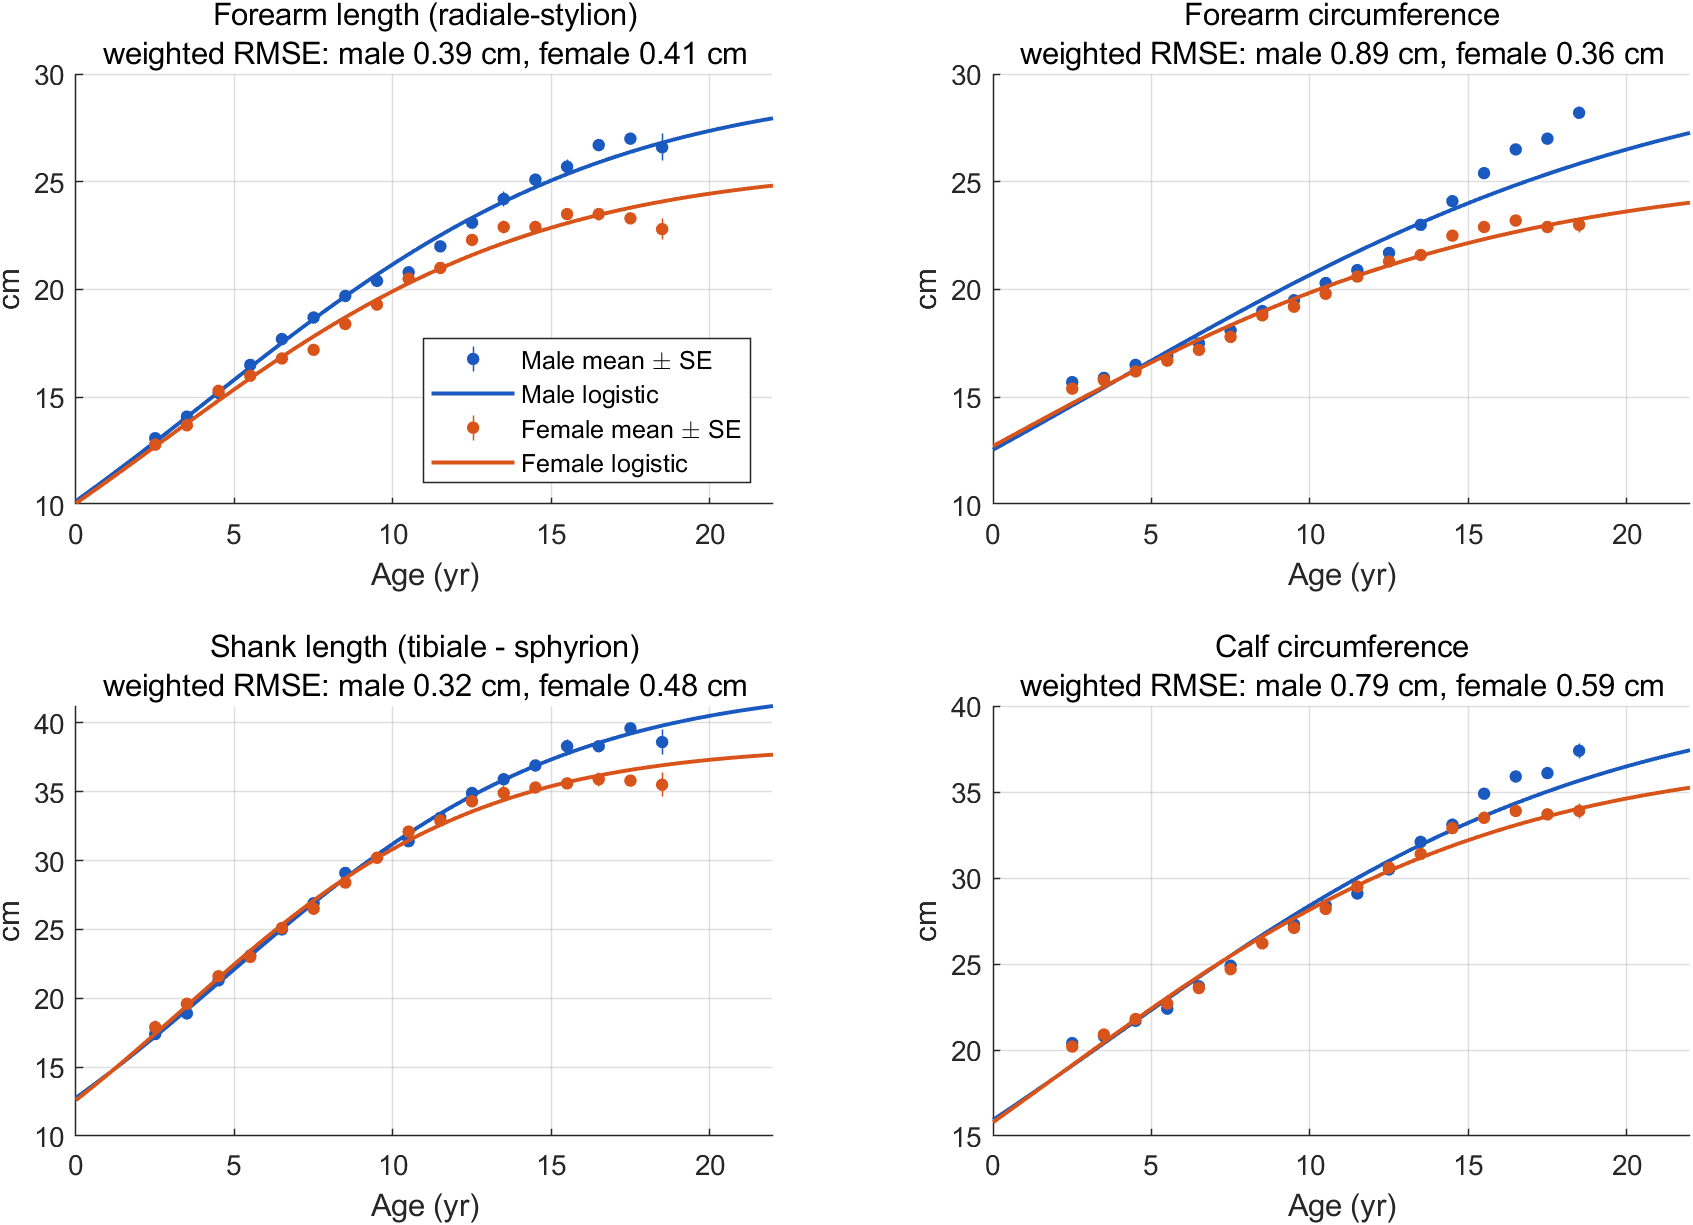
\includegraphics[width=0.92\textwidth]{growth_fits.png}
\caption{Snyder age-group means ($\pm$ standard error) and the logistic curves fitted to the individual records. The male forearm and calf circumferences rise above the curve at ages 13--18: the pubertal spurt.}
\label{fig:fits}
\end{figure}

\begin{remark}[growth spurt]\label{rem:spurt}
A single logistic curve cannot reproduce the pubertal spurt (ages 10--14 \cite{ghidini2025}). The largest misfit is male forearm circumference, which the curve underestimates by up to $2.4$\,cm at ages 15--18 (Figure~\ref{fig:fits}). Every later layer uses only the solution $x(a)$, so a two-phase curve is a drop-in replacement; Section~\ref{sec:spurt} uses one to measure how much the spurt changes $T^*$.
\end{remark}

\subsection{Two-phase growth: measuring the spurt}
\label{sec:spurt}
To test Remark~\ref{rem:spurt} we refit the arm curves as the sum of two logistic phases, childhood and puberty, under the same cap on adult size:
\begin{equation}
y(a)=\frac{K_1}{1+e^{-r_1(a-a_1)}}+\frac{K_2}{1+e^{-r_2(a-a_2)}} .
\label{eq:bilog}
\end{equation}
Equation~\eqref{eq:bilog} solves the sum of two logistic ODEs. Its threshold ages have no closed form, so they are found numerically by a bracketed root search on the increasing curve. Table~\ref{tab:spurt} shows that the second phase is real. It cuts the fit error by a factor of 2--6 to about the measurement noise, and it places the spurt at 13.6--14.8 years for boys and 10.3--10.4 years for girls, matching prosthetists' experience \cite{ghidini2025}.

\begin{table}[htbp]
\centering\small
\caption{Two-phase growth fits for the arm \eqref{eq:bilog}: $K$ in cm, $r$ in yr$^{-1}$, $a$ in yr; wRMSE in cm, as in Table~\ref{tab:fits}.}
\label{tab:spurt}
\setlength{\tabcolsep}{4pt}
\begin{tabular}{@{}llcccccccc@{}}
\toprule
Measurement & Sex & $K_1$ & $r_1$ & $a_1$ & $K_2$ & $r_2$ & $a_2$ (spurt) & wRMSE single & wRMSE two-phase\\
\midrule
Forearm length & M & 23.39 & 0.235 & 1.70 & 4.27 & 0.763 & 13.6 & 0.39 & 0.17\\
 & F & 17.13 & 0.467 & 0.36 & 6.34 & 0.644 & 10.3 & 0.41 & 0.19\\
Forearm circumference & M & 22.47 & 0.115 & $-4.14$ & 8.54 & 0.437 & 14.8 & 0.89 & 0.15\\
 & F & 16.66 & 0.203 & $-8.28$ & 7.17 & 0.363 & 10.4 & 0.36 & 0.15\\
\bottomrule
\end{tabular}
\end{table}

% =====================================================================
\section{Layer 2 --- the socket-fit map}
% =====================================================================

\subsection{Socket built at the fitting age}
At fitting age $a_0$ the socket is sized to the limb as it then is, with intentional oversize $s_C$ (prosthetists build loose and take up the slack with socks \cite{ghidini2025}) and distal clearance $\delta_0$:
\begin{equation}
C_s=(1+s_C)\,C(a_0),
\qquad
D_s=L(a_0)+\delta_0 .
\label{eq:socket}
\end{equation}

\subsection{Fit signals}
\begin{align}
\text{tightness:}\quad
\eps_c(a)&=\frac{C(a)-C_s}{C_s}
=\frac{C(a)}{(1+s_C)\,C(a_0)}-1,
\label{eq:epsc}\\[4pt]
\text{distal clearance:}\quad
\delta(a)&=D_s-L(a)=\delta_0-\rho\big[\lfa(a)-\lfa(a_0)\big].
\label{eq:delta}
\end{align}
At fitting $\eps_c=-s_C/(1+s_C)<0$ (loose, sock-filled) and $\delta=\delta_0>0$. Because $C$ and $L$ increase monotonically, $\eps_c$ rises and $\delta$ shrinks for all $a>a_0$.

% =====================================================================
\section{Layer 3 --- planar lift statics (a set of actions)}
\label{sec:lift}
% =====================================================================
The problem asks how the interface changes for a \emph{set} of actions as the child grows. We model a hold and a curl (and a reach in Section~\ref{sec:ext}), place the prosthesis mass and the held object at their own moment arms, and feed the curl's axial load back onto the clearance criterion.

\subsection{Free-body setup}
The residual forearm, socket and prosthesis form one rigid segment hinged at the elbow in the sagittal plane (Assumption~\ref{as:statics}). Let $\varphi$ be the forearm angle from the downward vertical ($\varphi=90^\circ$ is horizontal). Two weights act: the prosthesis weight $m_p g$ at its centre of mass, a distance $\ell_p$ from the elbow, and the object weight $m_o g$ at the terminal device, a distance $\ell_h$ from the elbow.

\begin{center}
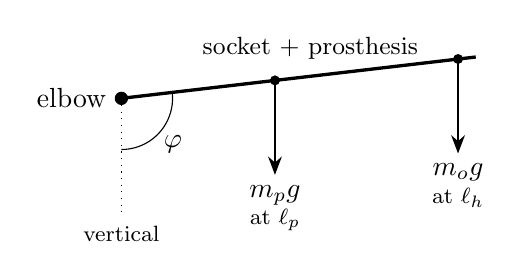
\begin{tikzpicture}[scale=1.5,>=Stealth]
  \coordinate (E) at (0,0);
  \coordinate (H) at (3,0.35);
  \coordinate (V) at (0,-1.0);
  \draw[dotted] (E) -- (V) node[below] {\footnotesize vertical};
  \pic[draw,angle radius=0.65cm,angle eccentricity=1.35,"$\varphi$"] {angle=V--E--H};
  \draw[very thick] (E) -- (H);
  \fill (E) circle (1.6pt) node[left=2pt] {elbow};
  \node[above] at (1.6,0.25) {\small socket + prosthesis};
  \coordinate (Pp) at (1.3,0.152);
  \fill (Pp) circle (1.2pt);
  \draw[->,thick] (Pp) -- ++(0,-0.8) node[below,align=center] {$m_p g$\\[-2pt]{\footnotesize at $\ell_p$}};
  \coordinate (Ph) at (2.85,0.333);
  \fill (Ph) circle (1.2pt);
  \draw[->,thick] (Ph) -- ++(0,-0.8) node[below,align=center] {$m_o g$\\[-2pt]{\footnotesize at $\ell_h$}};
\end{tikzpicture}
\end{center}

\subsection{Projection with separate moment arms}
The weight components perpendicular to the segment act at their own moment arms; the components along it give the axial load (sign: $+$ pull-off, $-$ push-on):
\begin{equation}
M_s=g\,\big(m_p\,\ell_p+m_o\,\ell_h\big)\sin\varphi,
\qquad
\Fax=(m_p+m_o)\,g\cos\varphi .
\label{eq:lift}
\end{equation}
For $\varphi>90^\circ$, $\cos\varphi<0$ and the load pushes the socket onto the limb. The arms $\ell_p$ and $\ell_h$ are \emph{fixed at the fitting age}: the prosthesis is built once and does not grow, so $M_s$ is constant over the socket's service life. We take $\ell_h$ as the measured elbow--hand length at $a_0$ \cite{snyder1977}; $\ell_p$ is not reported for children's prostheses, so we assume $\ell_p=0.5\,\ell_h$ and sweep $0.4$--$0.7\,\ell_h$ (segment tables scaled to child lengths \cite{otmani2023} could refine this). Neither arm affects $T^*$.

\subsection{Two actions}
\begin{center}
\small
\renewcommand{\arraystretch}{1.3}
\begin{tabular}{@{}L{3.0cm}cL{3.2cm}L{3.2cm}L{4.4cm}@{}}
\toprule
Action & $\varphi$ & Bending $M_s$ & Axial $\Fax$ & Boy fitted at 10, central masses\\
\midrule
A: hold (maximum bending) & $90^\circ$ & $g\,(m_p\ell_p+m_o\ell_h)$ & $0$ & $M_s=1.66$\,N\,m, $\Fax=0$\\
B: curl, hand to mouth & $150^\circ$ & $\tfrac12 g\,(m_p\ell_p+m_o\ell_h)$ & $-\tfrac{\sqrt3}{2}(m_p+m_o)g$ (push-on) & $M_s=0.83$\,N\,m, $\Fax=-4.84$\,N\\
\bottomrule
\end{tabular}
\end{center}
Action A isolates peak bending; action B produces a compressive load that pistons the socket onto the limb.

\subsection{Pistoning displacement from the curl}
In action B the compressive load drives the socket a distance $\lift$ onto the limb, resisted by the liner and soft-tissue axial stiffness $k_s$:
\begin{equation}
\boxed{\;\lift=\frac{|\Fax|}{k_s}
=\frac{(m_p+m_o)\,g\,|\cos\varphi_B|}{k_s}\;},
\qquad
|\cos\varphi_B|=\tfrac{\sqrt3}{2}.
\label{eq:ulift}
\end{equation}
With $k_s\approx75$\,N\,cm$^{-1}$ \cite{gholizadeh2011} and the mass ranges of Table~\ref{tab:vars}, $\lift=0.033$--$0.102$\,cm: about a millimetre at most. Pistoning of $0.5$\,cm would need $k_s\lesssim15$\,N\,cm$^{-1}$ with the heaviest load.

\begin{remark}[how much the lift matters]\label{rem:lift}
Through \eqref{eq:ulift} the lifted load enters the clearance criterion \eqref{eq:ad}, so heavier objects bring the threshold earlier. For a boy fitted at 10, $T^*$ falls from $20.2$ months with no load to $19.3$ months with the central load and $18.7$ months with the heaviest ($0.66$\,kg). The direction is robust; the size is small, because children's objects are light compared with the liner stiffness.
\end{remark}

% =====================================================================
\section{Layer 4 --- the replacement threshold}
\label{sec:threshold}
% =====================================================================

\subsection{Criteria}
An intervention is needed at the earliest age at which any of three criteria reaches tolerance (Assumption~\ref{as:trigger}). The clearance criterion fires once the limb, pistoned in by $\lift$, reaches the distal end of the socket:
\begin{align}
a^*_c:&\quad \eps_c(a)=\eps_{\max}, \label{eq:ac}\\
a^*_d:&\quad \delta(a)=\lift
\quad\Longleftrightarrow\quad L(a)=D_s-\lift , \label{eq:ad}\\
a^*_\ell:&\quad \Delta L(a)=\lfa(a)-\lfa(a_0)=\Delta L_{\max}, \label{eq:aell}\\
&\boxed{\,a^*=\min(a^*_c,\,a^*_d,\,a^*_\ell)\,},\qquad \boxed{\,T^*=12\,\pluspart{a^*-a_0}\ \text{months}\,}. \label{eq:astar}
\end{align}

\subsection{Analytic inversion}
\paragraph{Tightness.} Condition~\eqref{eq:ac} with \eqref{eq:epsc} gives the target circumference
\begin{equation}
C(a^*_c)=C_s(1+\eps_{\max})=(1+\Gamma)\,C(a_0)\;=:\;C_\tgt,
\qquad
\Gamma:=(1+s_C)(1+\eps_{\max})-1 .
\label{eq:Ctgt}
\end{equation}
Only the product $\Gamma$ enters, so $s_C$ and $\eps_{\max}$ can never be separated by outcome data. Inserting \eqref{eq:Csol},
\begin{equation}
1+B_C e^{-r_C(a-a_b)}=\frac{K_C}{C_\tgt}
\;\Rightarrow\;
e^{-r_C(a-a_b)}=\frac{1}{B_C}\!\left(\frac{K_C}{C_\tgt}-1\right),
\end{equation}
hence
\begin{equation}
\boxed{\;a^*_c=a_b-\frac{1}{r_C}\ln\!\left[\frac{1}{B_C}\!\left(\frac{K_C}{C_\tgt}-1\right)\right]\;}.
\label{eq:acsol}
\end{equation}
With $a_b=a_{50}$ and $u_0:=e^{-r_C(a_0-a_{50})}$, so that $C(a_0)=K_C/(1+u_0)$, this simplifies to an explicit service interval:
\begin{equation}
T^*_c=\frac{12}{r_C}\,\ln\!\frac{(1+\Gamma)\,u_0}{u_0-\Gamma}\ \text{months},
\qquad\text{finite iff}\quad u_0>\Gamma .
\label{eq:Tc}
\end{equation}

\paragraph{Clearance (with pistoning).} By \eqref{eq:rho}, condition~\eqref{eq:ad} reads $\rho[\lfa(a)-\lfa(a_0)]=\delta_0-\lift$, i.e.\ the intact forearm must grow by $(\delta_0-\lift)/\rho$:
\begin{equation}
\lfa(a^*_d)=\lfa(a_0)+\frac{\delta_0-\lift}{\rho}\;=:\;L_\tgt/\rho,
\qquad
L_\tgt=L(a_0)+\delta_0-\lift ,
\label{eq:Ltgt}
\end{equation}
and the same inversion on \eqref{eq:Lsol} yields
\begin{equation}
\boxed{\;a^*_d=a_b-\frac{1}{r_L}\ln\!\left[\frac{1}{B_L}\!\left(\frac{K_L}{L_\tgt}-1\right)\right]\;}.
\label{eq:adsol}
\end{equation}
The lift lowers $L_\tgt$ by $\lift$, so a heavier load fires the clearance criterion at a younger age.

\paragraph{Length discrepancy.} As the child grows, the intact arm lengthens while the prosthesis, built at $a_0$, does not; prosthetists identify this as a separate replacement driver \cite{ghidini2025}. With $\lfa(a)=K_\Lambda/[1+B_\Lambda e^{-r_\Lambda(a-a_b)}]$ and $B_\Lambda=(K_\Lambda-\lfa(a_b))/\lfa(a_b)$, condition~\eqref{eq:aell} gives
\begin{equation}
\lfa(a^*_\ell)=\lfa(a_0)+\Delta L_{\max}\;=:\;\Lambda_\tgt ,
\label{eq:Lamtgt}
\end{equation}
and the same inversion yields
\begin{equation}
\boxed{\;a^*_\ell=a_b-\frac{1}{r_\Lambda}\ln\!\left[\frac{1}{B_\Lambda}\!\left(\frac{K_\Lambda}{\Lambda_\tgt}-1\right)\right]\;}.
\label{eq:aellsol}
\end{equation}
The growing intact length $\lfa(a)$ drives this criterion, while its value \emph{at fitting} sets the fixed arm $\ell_h$ in \eqref{eq:lift}; the two uses are consistent and distinct.

\begin{proposition}[clearance versus length]\label{prop:race}
Criteria \eqref{eq:ad} and \eqref{eq:aell} are both crossings of the same increasing curve $\lfa(a)$, at heights $(\delta_0-\lift)/\rho$ and $\Delta L_{\max}$ above $\lfa(a_0)$. Hence, for every fitting age,
\[
a^*_d<a^*_\ell\iff\frac{\delta_0-\lift}{\rho}<\Delta L_{\max}.
\]
Which of the two fires first is a property of the socket design, not of the child's age.
\end{proposition}

\subsection{Edge cases and well-posedness}
\label{sec:edge}
\begin{enumerate}[label=\textbf{E\arabic*.},ref=E\arabic*,leftmargin=2.6em,itemsep=2pt]
\item \textbf{Target above the adult size.} The logarithms in \eqref{eq:acsol}, \eqref{eq:adsol} and \eqref{eq:aellsol} are real only if $C_\tgt<K_C$, $L_\tgt<K_L$ and $\Lambda_\tgt<K_\Lambda$. Otherwise the limb never reaches the target, that criterion never fires, and we set its age to $+\infty$. For tightness this gives an explicit cut-off fitting age,
\begin{equation}
a^{\max}_{0,c}=a_{50}-\frac{\ln\Gamma}{r_C}\qquad(\text{boys }16.2\text{ yr, girls }11.0\text{ yr at }\Gamma=0.255),
\label{eq:cutoff}
\end{equation}
and similarly for the other two. If all three ages are infinite, $T^*=\infty$: no growth-driven intervention before adulthood (the socket is then replaced for wear, outside this model).
\item \textbf{Socket loaded at fitting.} If $\delta_0\le\lift$, the limb end bears load on the first curl: $a^*_d=a_0$ and $T^*=0$. The design is infeasible; a larger $\delta_0$ or a stiffer liner is needed. Likewise $\Gamma=0$ gives $T^*_c=0$. The clamp $\pluspart{\cdot}$ in \eqref{eq:astar} keeps $T^*\ge0$.
\item \textbf{Ties.} If two criteria fire at the same age, $a^*$ is still well defined; only the label of the cause is ambiguous. Proposition~\ref{prop:race} shows that clearance and length tie only when $(\delta_0-\lift)/\rho=\Delta L_{\max}$.
\item \textbf{Very young fitting.} As $a_0$ decreases, $T^*_c$ in \eqref{eq:Tc} falls monotonically to the floor $(12/r_C)\ln(1+\Gamma)$ (25.3 months for boys at $\Gamma=0.255$), so tightness never fires faster than that. The length-type criteria are \emph{not} monotone below $a_{50}$: the absolute growth rate $\lfa'(a)$ peaks at $a_{50}$, so $T^*_d$ and $T^*_\ell$ are smallest for fitting near $a_{50}$ (2.7--4.2 yr for the forearm) and slightly longer below it (e.g.\ 21.0 months at age 2 against 20.8 at 3--4 for the length criterion in boys). Predictions are therefore reported only for $a_0\ge3$.
\item \label{ec:extrap}\textbf{Extrapolation.} Snyder data cover ages 2--18; ages beyond 18 are reached only through the fitted asymptote, which sits at the 10\% cap for six curves. Late-fitting predictions (ages 15--17), where $T^*$ grows steeply, are the most sensitive to this cap.
\item \textbf{Small or negative $a_{50}$.} Girls' forearm circumference has $a_{50}=0.07$ (and $-0.01$ in the first-pass fit to the age-group table): its inflection lies at birth. This is admissible, since \eqref{eq:a50} holds for any real $a_{50}$, and simply means the curve is already decelerating at all fitted ages.
\item \textbf{Range of $\rho$.} As $\rho\to0$ the residual limb stops growing and the clearance criterion never fires; $\rho>1$ is not physical. All sweeps use $0.2\le\rho\le1$.
\end{enumerate}

% =====================================================================
\section{Sensitivity analysis}
\label{sec:sens}
% =====================================================================

\subsection{Monotonicity in the design inputs}
The growth curves depend only on $\theta$, not on the socket design. Differentiating \eqref{eq:acsol} with $a^*_c=a_b-\frac1{r_C}\ln q$, $q=\frac1{B_C}(\frac{K_C}{C_\tgt}-1)$ and $B_Cq=\frac{K_C-C_\tgt}{C_\tgt}$ gives
\begin{equation}
\pd{a^*_c}{C_\tgt}
=\frac{K_C}{r_C\,C_\tgt\,(K_C-C_\tgt)}\;>0,
\label{eq:dacdCtgt}
\end{equation}
and since $C_\tgt=(1+s_C)(1+\eps_{\max})C(a_0)$,
\begin{equation}
\pd{a^*_c}{s_C}=\frac{K_C\,(1+\eps_{\max})\,C(a_0)}{r_C\,C_\tgt(K_C-C_\tgt)}>0,
\qquad
\pd{a^*_c}{\eps_{\max}}=\frac{K_C\,(1+s_C)\,C(a_0)}{r_C\,C_\tgt(K_C-C_\tgt)}>0 .
\label{eq:dac}
\end{equation}
Likewise, from \eqref{eq:Ltgt},
\begin{equation}
\pd{a^*_d}{L_\tgt}=\frac{K_L}{r_L\,L_\tgt(K_L-L_\tgt)}>0
\;\Rightarrow\;
\underbrace{\pd{a^*_d}{\delta_0}>0}_{\text{more clearance: later}},
\quad
\underbrace{\pd{a^*_d}{\lift}<0}_{\text{heavier lift: earlier}},
\quad
\underbrace{\pd{a^*_d}{\rho}<0}_{\text{faster residual growth: earlier}} ,
\label{eq:dad}
\end{equation}
and $\partial a^*_\ell/\partial\Delta L_{\max}>0$. Equations \eqref{eq:dac} and \eqref{eq:dad} show that \textbf{more oversize, tolerance or clearance always delays the threshold}, with no interior optimum. The largest sensible values are set by the clinical ceiling beyond which a loose socket degrades control \cite{ghidini2025}, a prescribed input rather than something the model selects. Monotonicity has a practical use: the extremes of $T^*$ over a box of inputs occur at its corners, so the bands below are exact, not sampled.

\subsection{Monotonicity in the fitting age}
Differentiating \eqref{eq:Tc} with respect to $u_0$,
\begin{equation}
\dd{}{u_0}\ln\!\frac{(1+\Gamma)u_0}{u_0-\Gamma}=\frac{1}{u_0}-\frac{1}{u_0-\Gamma}=\frac{-\Gamma}{u_0(u_0-\Gamma)}<0,
\end{equation}
and $u_0$ decreases with $a_0$, so $T^*_c$ \emph{increases strictly} with fitting age and diverges at the cut-off \eqref{eq:cutoff}. Children fitted older are further along the decelerating part of the curve, so a given relative tolerance takes longer to use up.

\subsection{\texorpdfstring{Headline result: $T^*$ versus fitting age for the arm}{Headline result: T* versus fitting age for the arm}}
\label{sec:headline}
We evaluate \eqref{eq:astar} for the arm with the final forearm curves (Table~\ref{tab:fits}) and the central constants of Table~\ref{tab:vars}: $\Gamma=0.255$ (final leg calibration; dimensionless, so it transfers by Assumption~\ref{as:transfer}), $\delta_0=1.5$\,cm, $\rho=1$, $\Delta L_{\max}=2$\,cm, $m_p=0.24$\,kg, $m_o=0.33$\,kg and $k_s=75$\,N\,cm$^{-1}$ ($\lift=0.065$\,cm). The band sets every uncertain input to its low or high end together: $\Gamma\in[0.147,0.260]$ (its 95\% CI), $\delta_0\in[1,3]$\,cm, $\rho\in[0.5,1]$, $\Delta L_{\max}\in[1,3]$\,cm, $\lift\in[0.033,0.102]$\,cm. By monotonicity, these corners bound $T^*$ over the whole box.

\begin{figure}[htbp]
\centering
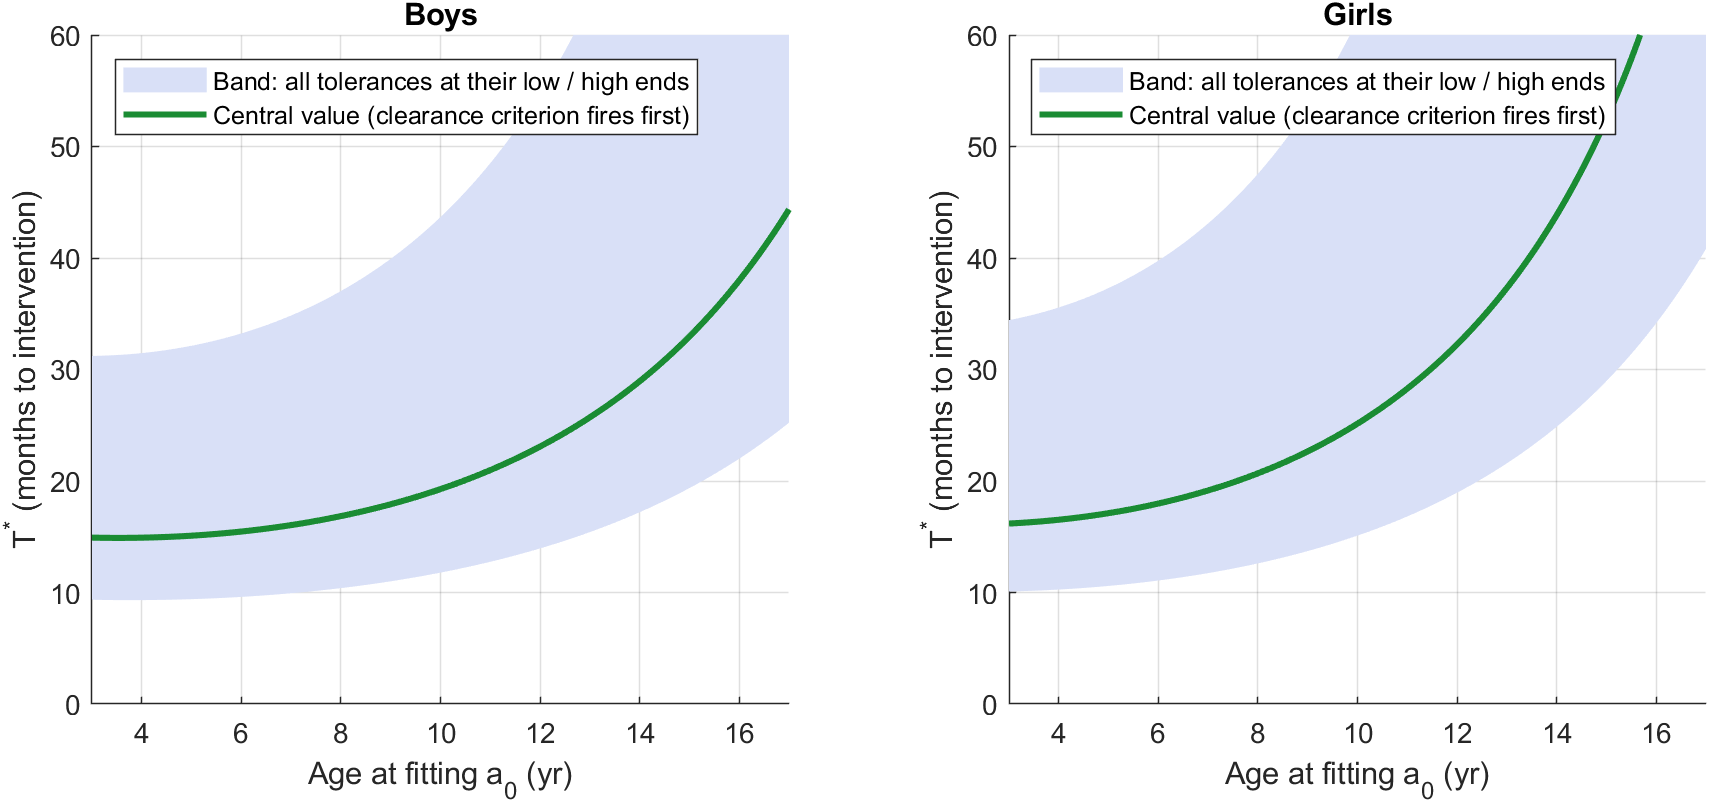
\includegraphics[width=\textwidth]{arm_headline.png}
\caption{Predicted months to the first growth-driven intervention for a below-elbow socket, by age at fitting, for the mean-tolerance child. Line: central constants; shading: all uncertain inputs at their low or high ends. At the central values, distal clearance fires first at every age.}
\label{fig:headline}
\end{figure}

\paragraph{Two kinds of uncertainty.} The band in Figure~\ref{fig:headline} is \emph{design and parameter} uncertainty. Children also differ from each other: the leg validation needs a child-to-child spread in every tolerance ($\sigma=0.63$ in the final fit, Section~\ref{sec:final}), and $\sigma$ is dimensionless, so it transfers to the arm (Assumption~\ref{as:transfer}). Table~\ref{tab:arm} therefore reports the mean-tolerance child (the deterministic formula), the median child with its confidence interval, and the spread over children when every uncertainty acts together. The tolerances are skewed and the earliest criterion wins, so the median child needs intervention sooner than the mean-tolerance child.

\begin{table}[htbp]
\centering\footnotesize
\setlength{\tabcolsep}{3.5pt}
\caption{Final arm prediction, $T^*$ in months (Section~\ref{sec:armfinal}). \emph{Median child}: central design values, with the 95\% confidence interval from 3,000 child and growth bootstrap draws. \emph{10--90\%}: spread over children when children, constants, growth curves and design ranges ($\delta_0$ 1--3\,cm, $\rho$ 0.5--1, $\Delta L_{\max}$ 1--3\,cm, $m_p$, $m_o$, $k_s$ 25--150\,N\,cm$^{-1}$) all vary. \emph{Mean tol.}: the deterministic formula at central values. Clearance fires first in every central case.}
\label{tab:arm}
\begin{tabular}{@{}c ccc ccc@{}}
\toprule
 & \multicolumn{3}{c}{Boys} & \multicolumn{3}{c}{Girls}\\
\cmidrule(lr){2-4}\cmidrule(l){5-7}
$a_0$ (yr) & Median child (95\% CI) & 10--90\% & Mean tol. & Median child (95\% CI) & 10--90\% & Mean tol.\\
\midrule
4  & 9.8 (6.0--12.4)   & 4.9--24.1  & 14.9 & 10.7 (6.5--13.7)  & 5.4--27.0  & 16.5\\
6  & 10.1 (6.2--12.8)  & 5.0--25.4  & 15.5 & 11.6 (7.2--14.9)  & 5.8--30.2  & 18.0\\
8  & 10.9 (6.7--13.9)  & 5.4--28.1  & 16.9 & 13.2 (8.1--17.1)  & 6.6--35.9  & 20.7\\
10 & 12.3 (7.6--15.8)  & 6.1--32.6  & 19.3 & 15.8 (9.7--20.7)  & 7.8--44.7  & 25.1\\
12 & 14.5 (8.9--18.7)  & 7.1--39.7  & 23.1 & 19.9 (11.9--26.5) & 9.6--60.3  & 32.3\\
14 & 17.8 (10.7--23.2) & 8.6--50.8  & 28.9 & 25.9 (15.3--36.2) & 12.3--89.2 & 43.8\\
16 & 22.6 (13.4--29.9) & 10.8--69.1 & 38.0 & 35.4 (20.1--53.9) & 16.3--172  & 64.2\\
\bottomrule
\end{tabular}
\end{table}

\paragraph{Reading the result.} A typical child fitted between 4 and 10 needs intervention after a median of 10--12 months (boys) or 11--16 months (girls). This is close to the 11.8-month median observed in the leg casefiles and between the 8.3-month adjustment and 16.4-month replacement intervals reported clinically \cite{ghidini2025}. One child in ten needs intervention within about 5--8 months, and one in ten lasts roughly two years or longer. The interval lengthens after puberty, and faster for girls, whose growth ends earlier. At the central values the clearance criterion fires first because the intact forearm grows about 1\,cm per year, using up $(\delta_0-\lift)/\rho\approx1.4$\,cm in under two years, whereas the 25\% circumference tolerance takes five years or more (and is never reached by boys fitted after 16.2 or girls fitted after 11.0, eq.~\eqref{eq:cutoff}).

\subsection{Which unknown matters most}
\label{sec:tornado}
\begin{figure}[htbp]
\centering
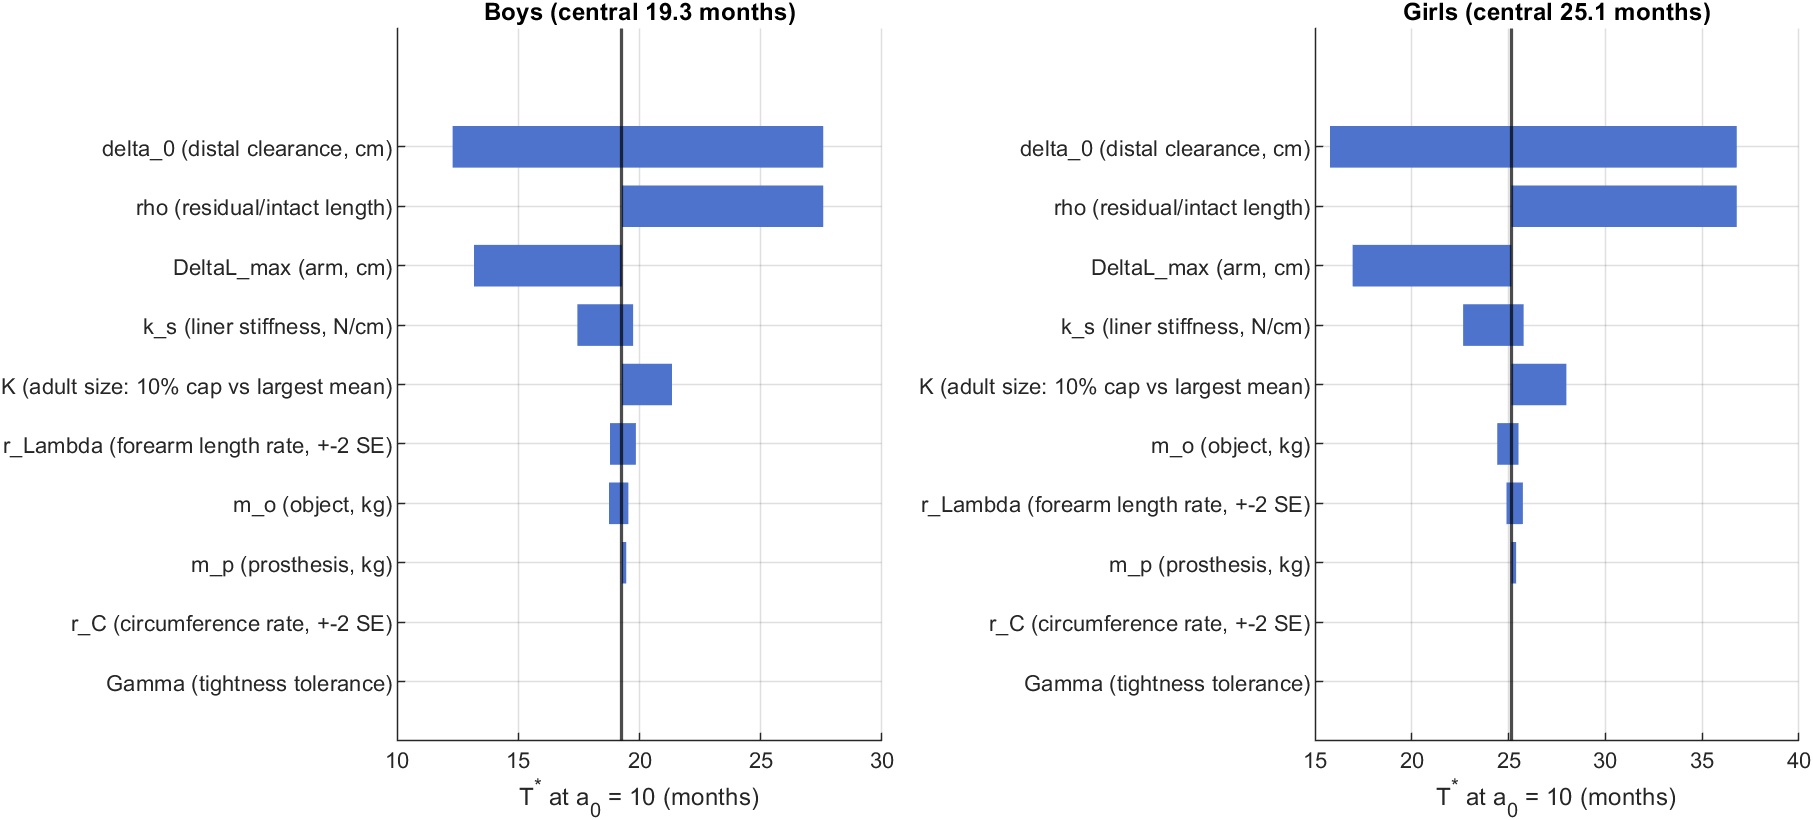
\includegraphics[width=\textwidth]{arm_tornado.png}
\caption{One-at-a-time sensitivity of $T^*$ for a child fitted at 10 (mean-tolerance child). Each bar moves one input across its range with all others central.}
\label{fig:tornado}
\end{figure}
Figure~\ref{fig:tornado} moves each uncertain input across its range with the others held central. The distal clearance $\delta_0$ dominates: from 1 to 3\,cm it moves $T^*$ from 12 to 28 months (boys) and from 16 to 37 months (girls). Next come $\rho$ and the arm $\Delta L_{\max}$. The liner stiffness matters only if it is much softer than measured ($k_s=25$\,N\,cm$^{-1}$ costs 2--3 months). The cap on adult size moves $T^*$ by 2--3 months, and the growth-rate uncertainty and the masses by about 1. $\Gamma$ has no effect at age 10, because tightness is not the first criterion there. So the most valuable single measurement for arm sockets is the clearance prosthetists build in, followed by the residual-to-intact growth ratio $\rho$. The variance-based analysis of Section~\ref{sec:sobol}, which varies all inputs together, adds the arm length tolerance as an equally important unknown.

\paragraph{A leg-informed scenario.} The final leg fit (Section~\ref{sec:final}) implies that the leg clearance closes after 1.60\,cm of intact growth for the mean child. If the arm behaved the same way ($\rho\approx0.94$ with $\delta_0=1.5$\,cm), clearance would still fire first and the mean-tolerance $T^*$ would rise by only 1--2 months for fitting ages 4--10 (boys 15.9--20.6, girls 17.7--27.0 months). The leg data therefore support the central arm values. The first-pass competing-risks fit (2.9\,cm, Section~\ref{sec:cr}) would have implied $\rho\approx0.52$ and much longer intervals, which shows why measuring $\rho$ for the arm still matters.

\subsection{Effect of the growth spurt}
\label{sec:spurteffect}
\begin{figure}[htbp]
\centering
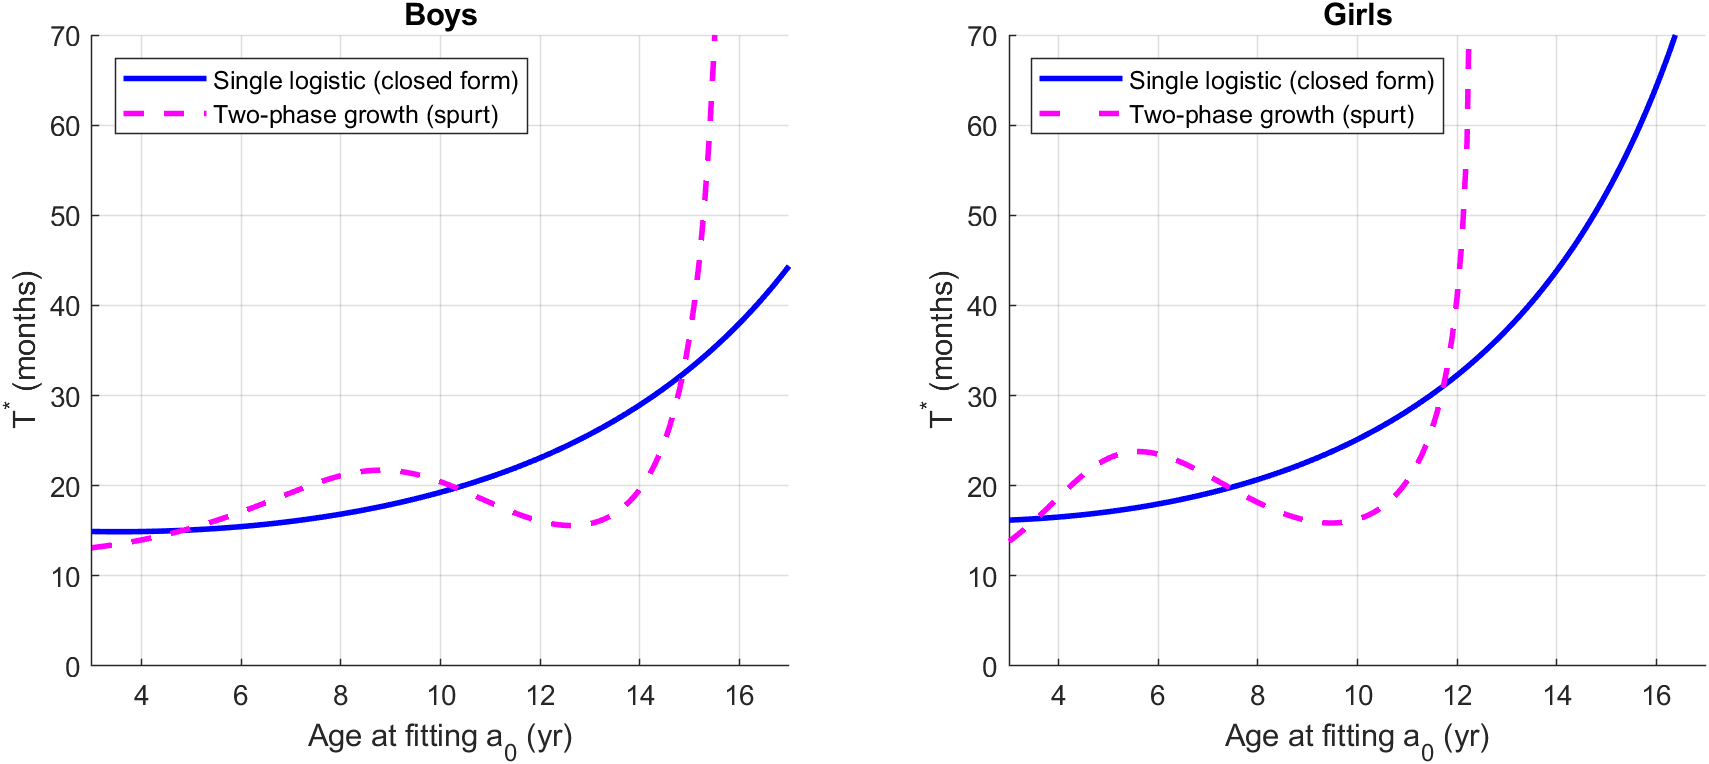
\includegraphics[width=\textwidth]{arm_growth_spurt.png}
\caption{Mean-tolerance $T^*$ with the single logistic (closed form) and with the two-phase growth curves of Table~\ref{tab:spurt}.}
\label{fig:spurt}
\end{figure}
With the two-phase curves (Figure~\ref{fig:spurt}), the smooth rise of $T^*$ with fitting age becomes the dip anticipated in Remark~\ref{rem:spurt}. Fitting just before the spurt shortens the interval by up to 9 months: boys fitted at 12--14 need intervention after 16--20 instead of 23--29 months, and girls fitted at 10 after 16 instead of 25 months. Fitting in mid-childhood (ages 4--9) lengthens it by up to 6 months, because the two-phase curve grows more slowly than the single logistic there. Fitting after the spurt lengthens it sharply. Girls fitted after about 12.5 and boys fitted after about 16 reach no growth-driven threshold at all, because their measured forearm length has less than the 1.4\,cm of growth left that would close the clearance. The late-fitting values of the single logistic for girls therefore come partly from the 10\% cap on adult size (edge case~\ref{ec:extrap}). The single logistic remains the analytic backbone and is what was validated on the leg. For children fitted within about two years before the spurt, the two-phase prediction is the better guide.

\subsection{Definition of ``substantial change''}
The point of substantial change is $a^*=\min(a^*_c,a^*_d,a^*_\ell)$: the earliest age at which the socket becomes intolerably tight ($\eps_c=\eps_{\max}$), the limb end begins bearing load on every curl ($\delta=\lift$), or the length discrepancy with the intact arm reaches tolerance ($\Delta L=\Delta L_{\max}$). $T^*$ is the predicted service interval of the socket.

% =====================================================================
\section{Validation against clinical data}
\label{sec:validation}
% =====================================================================

This section is the first-pass validation, built on the data-pack episode table with stand-in fitting ages. Section~\ref{sec:final} repeats it with per-child records; its values are final and supersede the ones below where they differ.

\subsection{Data}
The only paediatric casefile data available are for the leg: 62 Cambodian children with transtibial (TT), knee-disarticulation (KD) or transfemoral (TF) limb loss, with 814 dated visits \cite{ghidiniData}; 59 of them contribute at least one socket episode. We split each child's history into socket episodes. An episode starts at a new prosthesis. It ends in an \emph{event} at the first later visit coded as a growth problem (``socket tight'' and/or ``short''), or is \emph{censored} at the next non-growth replacement or the last visit. Episodes of zero length are dropped. This gives 273 episodes (TT 188, KD 20, TF 65) with 155 events: 73 tight, 51 short and 31 both. The Kaplan--Meier median time to the first growth problem is 11.8 months, and 48\% of sockets are still problem-free at 12 months.

\subsection{Proxy assumption and design of the test}
Legs and arms grow differently, so comparing the arm model with leg intervals would test nothing. We therefore separate a \emph{structural test}, run on the leg where data exist, from the \emph{prediction}, run on the arm (Assumption~\ref{as:transfer}):
\begin{enumerate}[leftmargin=2.2em,itemsep=2pt]
\item \textbf{Leg model.} Replace the forearm curves by the Snyder shank-length and calf-circumference fits (Table~\ref{tab:fits}). Set $\lift=0$, since the arm lifts do not apply to walking.
\item \textbf{Simulated cohort.} The casefiles record no fitting ages, so $a_0$ is drawn from the 45 recorded ages at amputation (with Gaussian jitter of SD 0.5\,yr, kept within 2--18), and sex from the cohort mix (73\% boys). Child-to-child variation in tolerances is lognormal with log-SD $\sigma$. For 20,000 simulated sockets, $T^*$ follows from \eqref{eq:astar}, and the model survival curve is $S_{\mathrm{mod}}(t)=\Pr(T^*>t)$.
\item \textbf{Observed curve.} The Kaplan--Meier estimate, which accounts for right-censoring,
\begin{equation}
\widehat{S}(t)=\prod_{t_i\le t}\!\left(1-\frac{d_i}{n_i}\right),
\label{eq:km}
\end{equation}
where $d_i$ problems occur among the $n_i$ sockets still in service at $t_i$. It is evaluated monthly up to the last month with at least 10 sockets at risk: 25 months for TT and 18 for KD+TF.
\item \textbf{Score.} $\mathrm{RMSE}=\big[\frac1{N}\sum_t(S_{\mathrm{mod}}(t)-\widehat S(t))^2\big]^{1/2}$ and $R^2=1-\sum(\widehat S-S_{\mathrm{mod}})^2/\sum(\widehat S-\overline{S})^2$.
\item \textbf{Calibrate on TT, test on KD+TF.} The KD+TF episodes are never used in fitting.
\end{enumerate}

\subsection{Identifiability and calibration}
\label{sec:calib}
Two structural facts limit what the casefiles can determine. First, only $\Gamma=(1+s_C)(1+\eps_{\max})-1$ enters the tightness criterion \eqref{eq:Ctgt}. Second, with $\lift=0$, clearance and length are crossings of the same intact-shank curve (Proposition~\ref{prop:race}), so only $\lambda=\min(\delta_0/\rho,\Delta L_{\max})$ affects timing. The calibration therefore fits three constants $(\Gamma,\lambda,\sigma)$. It first sweeps a $40\times39\times11$ grid (17,160 sets), then refines with Nelder--Mead restarts until successive RMSEs differ by less than 0.01\% (ratio $\ge0.9999$). It converged at the third refinement:
\[
\Gamma=0.121,\qquad \lambda=1.95\text{ cm},\qquad \sigma=0.77 .
\]
Both physical constants lie inside independent literature ranges: $\Gamma$ within 0.005--0.26 \cite{volume1,patent,sanders2017,ghidiniPoster} and $\lambda$ within 0.5--2\,cm \cite{ghidini2025,ghidiniPoster}. Here $\Gamma$ is the combination of sock oversize $s_C\approx0.04$--$0.06$ and tolerance $\eps_{\max}\approx0.06$--$0.08$. The model reproduces real clinical data with physically plausible tolerances.

\subsection{Results}
\begin{table}[htbp]
\centering\small
\caption{Model versus Kaplan--Meier curves. The noise floor is the RMSE between bootstrap resamples of the TT episodes and their own Kaplan--Meier curve (1,000 resamples; 95\% range 0.015--0.074).}
\label{tab:rmse}
\begin{tabular}{@{}lcccc@{}}
\toprule
Comparison & Episodes & Free constants & RMSE & $R^2$\\
\midrule
TT, calibration & 188 & 3 & \textbf{0.0165} & \textbf{0.9963}\\
KD+TF, held out (TT constants) & 85 & 0 & \textbf{0.0293} & \textbf{0.9870}\\
TT without child-to-child spread ($\sigma=0$) & 188 & 2 & 0.0926 & 0.8839\\
TT, every constant free (7 constants) & 188 & 7 & 0.0155 & 0.9967\\
KD+TF refitted on itself (reference only) & 85 & 3 & 0.0188 & 0.9947\\
Noise floor, TT bootstrap (median) & 188 & -- & 0.0324 & 0.9858\\
\bottomrule
\end{tabular}
\end{table}

\begin{figure}[htbp]
\centering
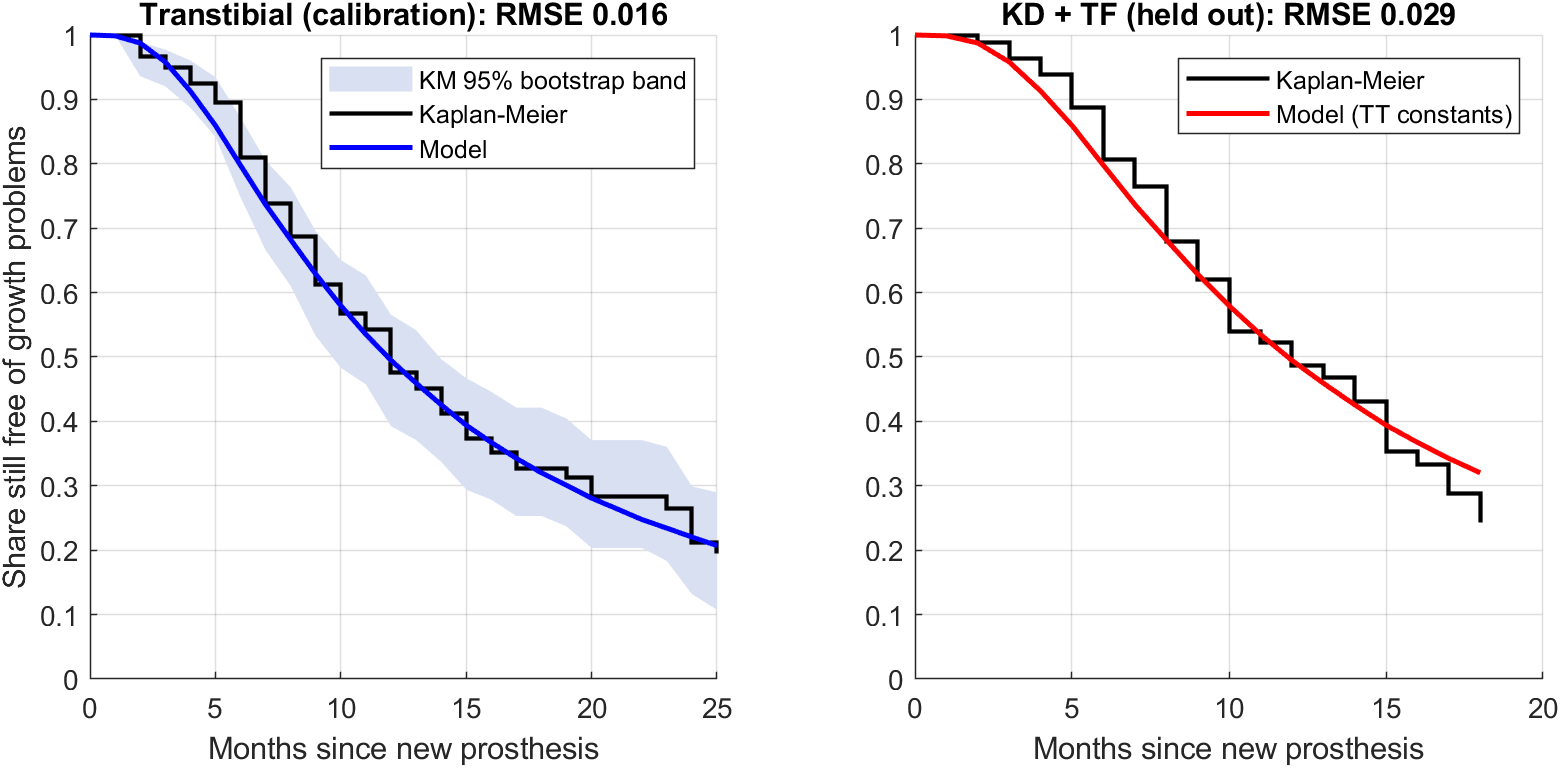
\includegraphics[width=\textwidth]{first_pass_km_vs_model.png}
\caption{Leg validation. Left: transtibial episodes used for calibration, with the 95\% bootstrap band of the Kaplan--Meier curve. Right: held-out knee-disarticulation and transfemoral episodes predicted with the transtibial constants.}
\label{fig:km}
\end{figure}

The calibrated model follows the observed curve within its sampling noise (Table~\ref{tab:rmse}, Figure~\ref{fig:km}). More importantly, it predicts the held-out amputation levels with an RMSE of 0.029, inside the bootstrap noise range, without any refitting. Fitting those levels directly lowers the RMSE only to 0.019.

\subsection{Is the fit meaningful? Benchmarks}
\label{sec:bench}
Any smooth decreasing curve scores a high $R^2$ against a survival curve, so $R^2$ alone flatters a model. Table~\ref{tab:bench} compares the growth model with two purely statistical survival curves fitted the same way: an exponential (constant hazard) and a Weibull. It also reports two stricter measures: the largest deviation from the Kaplan--Meier curve, and the share of months in which the model lies inside the 95\% bootstrap band of the data.

\begin{table}[htbp]
\centering\small
\setlength{\tabcolsep}{4pt}
\caption{Growth model versus statistical benchmarks, all fitted to the TT Kaplan--Meier curve. ``In band'': share of the 26 monthly points inside the 95\% bootstrap band.}
\label{tab:bench}
\begin{tabular}{@{}lccccccc@{}}
\toprule
Model & Constants & RMSE TT & $R^2$ TT & Max.\ dev. & In band & RMSE KD+TF & $R^2$ KD+TF\\
\midrule
Exponential & 1 & 0.060 & 0.952 & 0.144 & 77\% & 0.079 & 0.905\\
Weibull & 2 & 0.035 & 0.983 & 0.075 & 85\% & 0.048 & 0.965\\
Growth model, timing fit & 3 & \textbf{0.016} & \textbf{0.996} & \textbf{0.035} & \textbf{96\%} & \textbf{0.029} & \textbf{0.987}\\
Growth model, competing risks & 4 & 0.020 & 0.995 & 0.057 & 92\% & 0.035 & 0.982\\
\bottomrule
\end{tabular}
\end{table}

The growth model halves the Weibull error on the calibration set and still beats it on the held-out set, so the mechanism adds predictive power beyond curve fitting. It stays inside the data's 95\% band in 25 of 26 months.

\subsection{Which problem occurs: competing risks}
\label{sec:cr}
The timing fit cannot say whether clearance or length fires first: with $\lift=0$ both are crossings of the same curve (Proposition~\ref{prop:race}), and their thresholds collapse into one constant $\lambda$. The casefiles record \emph{which} problem occurred, so we also fit the model to the \emph{cumulative incidence} of each problem. This competing-risks extension of the Kaplan--Meier estimate (the Aalen--Johansen estimator) handles censoring correctly:
\begin{equation}
\widehat F_k(t)=\sum_{t_i\le t}\widehat S(t_i^-)\,\frac{d_{k,i}}{n_i},\qquad k\in\{\text{tight},\text{short}\}.
\label{eq:aj}
\end{equation}
Distal contact is not coded separately in the casefiles, and prosthetists treat it as socket tightness, relieving it by heating out the distal end of the socket or removing distal padding \cite{ghidini2025}. We therefore map the model's tightness \emph{and} clearance events to ``tight'' and its length events to ``short''. Events coded ``tight+short'' count half to each; assigning them wholly to one side instead is reported below. The tightness, clearance and length thresholds now have separate constants, $(\Gamma,\ \delta_0/\rho,\ \Delta L_{\max},\ \sigma)$, with an independent child-to-child draw for each criterion.

\begin{figure}[htbp]
\centering
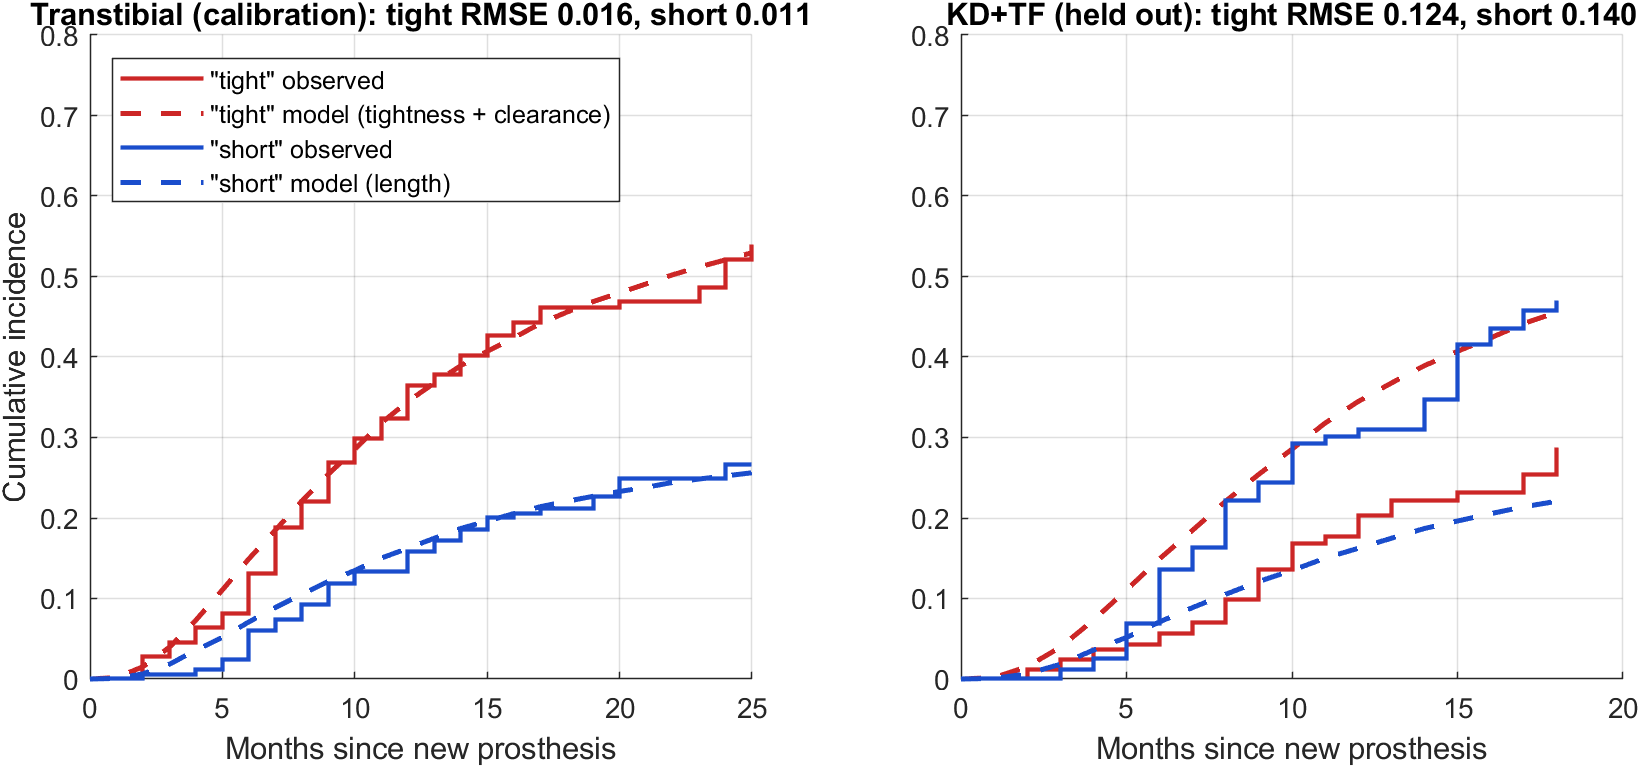
\includegraphics[width=\textwidth]{first_pass_competing_risks.png}
\caption{Cumulative incidence of tight and short problems: observed (steps) and competing-risks model (dashed). Left: transtibial calibration. Right: held-out knee-disarticulation and transfemoral episodes.}
\label{fig:cr}
\end{figure}

On the transtibial episodes the fit reproduces both incidence curves, with RMSE 0.016 (tight) and 0.011 (short) (Figure~\ref{fig:cr}). Overall survival keeps RMSE 0.020 ($R^2=0.995$). By 25 months 54\% of sockets have had a tight problem and 27\% a short one; the model attributes first problems almost equally to tightness (35\%), clearance (32\%) and length (33\%). Together, tightness and clearance give the observed two-thirds ``tight''. By contrast, the timing-only constants tie clearance and length exactly. They therefore predict no ``short'' problems at all (cause RMSE 0.17 for both curves), even though their overall survival fit is better. The competing-risks constants are
\[
\Gamma=0.124,\qquad \delta_0/\rho=4.6\text{ cm},\qquad \Delta L_{\max}=4.6\text{ cm},\qquad \sigma=0.98 ,
\]
as means over children (medians 2.9\,cm for the two lengths). $\Gamma$ agrees with the timing fit (0.121). With real fitting ages, the final fit places it higher and bounds it only from below (Section~\ref{sec:final}), which does not affect the arm. Across codings of the ``both'' events, $\Gamma$ stays in 0.10--0.14. The length tolerance is the weak point. A median of 2.9\,cm is above the 1\,cm prosthetists can fix with an ankle block and above the 2\,cm shortening seen clinically \cite{ghidini2025,ghidiniPoster}. ``Short'' may therefore be recorded only once the discrepancy is clearly visible, or growth may be faster in Cambodian children than in the Snyder curves. The final per-child fit (Section~\ref{sec:final}) resolves this: with real fitting ages the median-child tolerance falls to 1.85\,cm, inside the clinical range.

On the held-out levels, the overall timing is still predicted (RMSE 0.035, $R^2=0.982$), but the split between causes is not. The held-out group is dominated by transfemoral sockets (65 of 85 episodes), which fail mainly through length. This agrees with prosthetists' observation that transfemoral sockets are less prone to tightness \cite{ghidini2025}, and with their different socket design (ischial containment, not patellar-tendon bearing). Cause-specific tolerances are level-specific and should not be transferred between amputation levels.

\subsection{\texorpdfstring{Why $R^2=0.9999$ is not attainable}{Why R2 = 0.9999 is not attainable}}
\label{sec:r2}
$R^2=0.9999$ on the TT curve would require RMSE $\le0.0027$, about one twelfth of the noise floor. Bootstrap resamples of the TT data agree with their own Kaplan--Meier curve only to a median $R^2$ of $0.986$, so no model can honestly claim more. A model that matched the curve to $R^2=0.9999$ would be fitting the random steps of 188 episodes, not growth. Freeing every constant confirms this: seven constants (separate spreads, a clinic-visit delay, a fitting-age shift) raise $R^2$ only from 0.9963 to 0.9967. To get there the fit pushes $\Gamma$ to the top of its literature range and moves the fitting ages 4.5 years later. The first pass therefore kept the three-constant model. The final per-child study confirms the limit: its child-level noise floor is RMSE 0.033 (median), and the final five-constant model, at RMSE 0.0150 ($R^2=0.997$), already sits below it (Table~\ref{tab:finalmetrics}).

\subsection{Constants the data cannot fix}
\label{sec:sweep}
\begin{figure}[htbp]
\centering
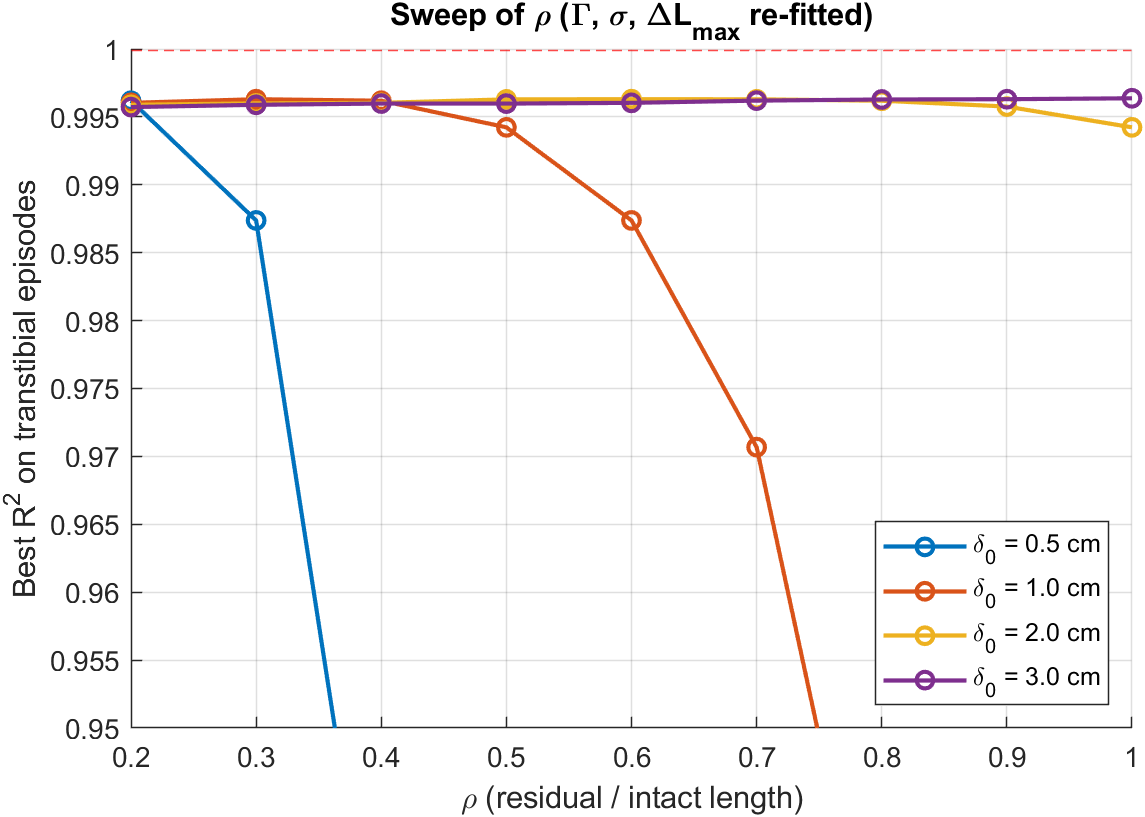
\includegraphics[width=0.62\textwidth]{first_pass_rho_sweep.png}
\caption{Best attainable $R^2$ on the TT episodes as $\rho$ varies, for four clearances $\delta_0$ ($\Gamma$ and $\sigma$ re-fitted at every point, best $\Delta L_{\max}$ on the grid). The fit is flat in $\rho$ as long as $\delta_0/\rho\gtrsim1.7$\,cm.}
\label{fig:rho}
\end{figure}
A sweep of $\rho\in[0.2,1]\times\delta_0\in\{0.5,1,2,3\}$\,cm$\,\times\,\Delta L_{\max}\in[0.5,3]$\,cm, with $\Gamma$ and $\sigma$ re-fitted at each of the 216 points, keeps the best $R^2$ between 0.9962 and 0.9964 for every $\rho$ (Figure~\ref{fig:rho}). The casefiles therefore constrain only the ratio $\delta_0/\rho$, not $\rho$ itself. With stand-in ages this first pass needed $\delta_0/\rho\gtrsim1.7$\,cm. The final per-child fit estimates it directly, at 1.60\,cm (95\% CI 1.16--3.04, Table~\ref{tab:final}), so $\rho\approx\delta_0/1.60$ for the leg: about 0.3 if $\delta_0=0.5$\,cm, 0.6 if $\delta_0=1$\,cm and 1 if $\delta_0=1.6$\,cm (the CI allows $\delta_0$ up to about 3\,cm at $\rho=1$). The prosthesis centre of mass $\ell_p$ and the arm tolerance $\Delta L^{\mathrm{arm}}_{\max}$ do not enter the leg model at all, so no fit to leg data can determine them. They remain literature or assumed inputs, carried in the band of Figure~\ref{fig:headline}.

\subsection{Robustness and an honest mismatch}
\begin{itemize}[leftmargin=1.4em,itemsep=2pt]
\item \textbf{Fitting-age stand-in.} Shifting the stand-in ages by $+1$, $+2$ or $+3$ years leaves the RMSE between 0.0155 and 0.0165 (TT) and between 0.027 and 0.029 (KD+TF). The constants move along a valley ($\Gamma$ 0.07--0.18, $\lambda$ 1.1--1.95\,cm), so they are only weakly identified individually.
\item \textbf{Child-to-child spread is essential.} Without $\sigma$ the RMSE rises to 0.093: one deterministic tolerance cannot produce both the early and the late problems. This matches the prosthetists' report that every child grows at a different rate \cite{ghidini2025}.
\item \textbf{Which criterion fires.} The timing fit alone cannot tell clearance from length; the competing-risks fit of Section~\ref{sec:cr} resolves this for transtibial sockets but not across amputation levels.
\end{itemize}

% =====================================================================
\section{Final validation with per-child records}
\label{sec:final}
% =====================================================================
Section~\ref{sec:validation} used the episode table of the data pack, with ages at amputation standing in for fitting ages. For the final values we went back to the raw sources and repeated the whole calibration with real per-episode ages, child-level resampling and out-of-sample tests. The values in this section supersede those of Section~\ref{sec:validation}.

\subsection{Data upgrades}
\begin{itemize}[leftmargin=1.4em,itemsep=1pt]
\item \textbf{Raw casefiles} \cite{ghidiniData}: the 814 dated visits were re-split into episodes with the same rules, reproducing the 273 episodes and 155 events exactly, but now with \emph{child identifiers} (59 children) and dates. For the 196 episodes whose child has a recorded age at amputation, the fitting age is
\[
a_0=\text{age at amputation}+\text{delay}+\text{years since the child's first clinic visit},
\]
with the delay a fitted constant; for the others it is drawn from the recorded ages. The sex mix is now level-specific (boys: TT 62\%, KD 83\%, TF 86\%).
\item \textbf{Snyder individual records} \cite{anthrokids}: the 3,895 children aged 2--18 replace the age-group table. All growth curves are refitted from individual records, including thigh length, whole-leg length and upper-thigh circumference, and every curve is bootstrapped 2,000 times by resampling children.
\item \textbf{NHANES} 1999--2000 and 2017--2020 \cite{nhanes}: modern calf and thigh circumferences (ages 8--19) as an independent growth source.
\item \textbf{IMPRINT} finite-element dataset \cite{imprint}: its residual-limb model uses soft-tissue and silicone-liner moduli of 0.25 and 0.6\,MPa. A shear estimate from these makes the tissue far stiffer than the clinical 75\,N\,cm$^{-1}$, which is dominated by liner--socket slip, so $\lift$ is at most about 1\,mm under either value.
\end{itemize}
The other datasets of the literature survey (EMG, kinematics, grasp-and-lift, residual-limb shape scans) do not inform any constant of this model and were not used.

\subsection{Protocol}
The study ran for 3.6 hours on 10 parallel workers:
\begin{enumerate}[leftmargin=2em,itemsep=1pt]
\item a sweep of 967,680 parameter sets;
\item multi-start Nelder--Mead refinement until successive RMSEs differed by less than 0.01\%;
\item 5,250 \emph{child-level} bootstrap refits, which resample whole children because episodes of the same child are not independent;
\item leave-one-child-out cross-validation over the 32 transtibial children;
\item ten model variants, each with 160--400 bootstrap refits;
\item 1,500 refits on bootstrapped growth curves.
\end{enumerate}
The model is the competing-risks version of Section~\ref{sec:cr}, with a child-level spread $\sigma$, fitted to the survival curve and both cause-specific incidence curves together (stacked RMSE), using 400 Monte Carlo draws per episode during fitting and 4,000 for the final evaluation. $\Gamma$ is kept within its literature range ($\le0.26$); an unbounded fit is reported as a variant.

\subsection{Final constants}
\begin{table}[htbp]
\centering\small
\caption{Final leg constants. Child bootstrap: 2.5\%, 50\%, 97.5\% over 5,250 refits on resampled children. Growth bootstrap: same over 1,500 refits on resampled growth curves.}
\label{tab:final}
\setlength{\tabcolsep}{4pt}
\begin{tabular}{@{}lcccc@{}}
\toprule
Constant & Estimate & Child bootstrap 95\% & Growth bootstrap 95\% & Literature\\
\midrule
$\Gamma$, tightness tolerance & 0.255 & 0.147--0.260 & 0.197--0.260 & 0.005--0.26\\
$\delta_0/\rho$, clearance (cm, mean child) & 1.60 & 1.16--3.04 & 1.43--1.75 & $\ge\delta_0=0.5$--3\\
$\Delta L_{\max}$, leg length tolerance (cm, mean child) & 2.26 & 1.50--4.51 & 1.95--2.50 & $\approx1$--2\\
$\sigma$, child-to-child spread & 0.63 & 0.43--0.96 & 0.56--0.69 & --\\
delay, amputation to first visit (yr) & 0.0001 & 0.0000--0.0002 & 0.0001--0.0001 & --\\
\bottomrule
\end{tabular}
\end{table}
\begin{figure}[htbp]
\centering
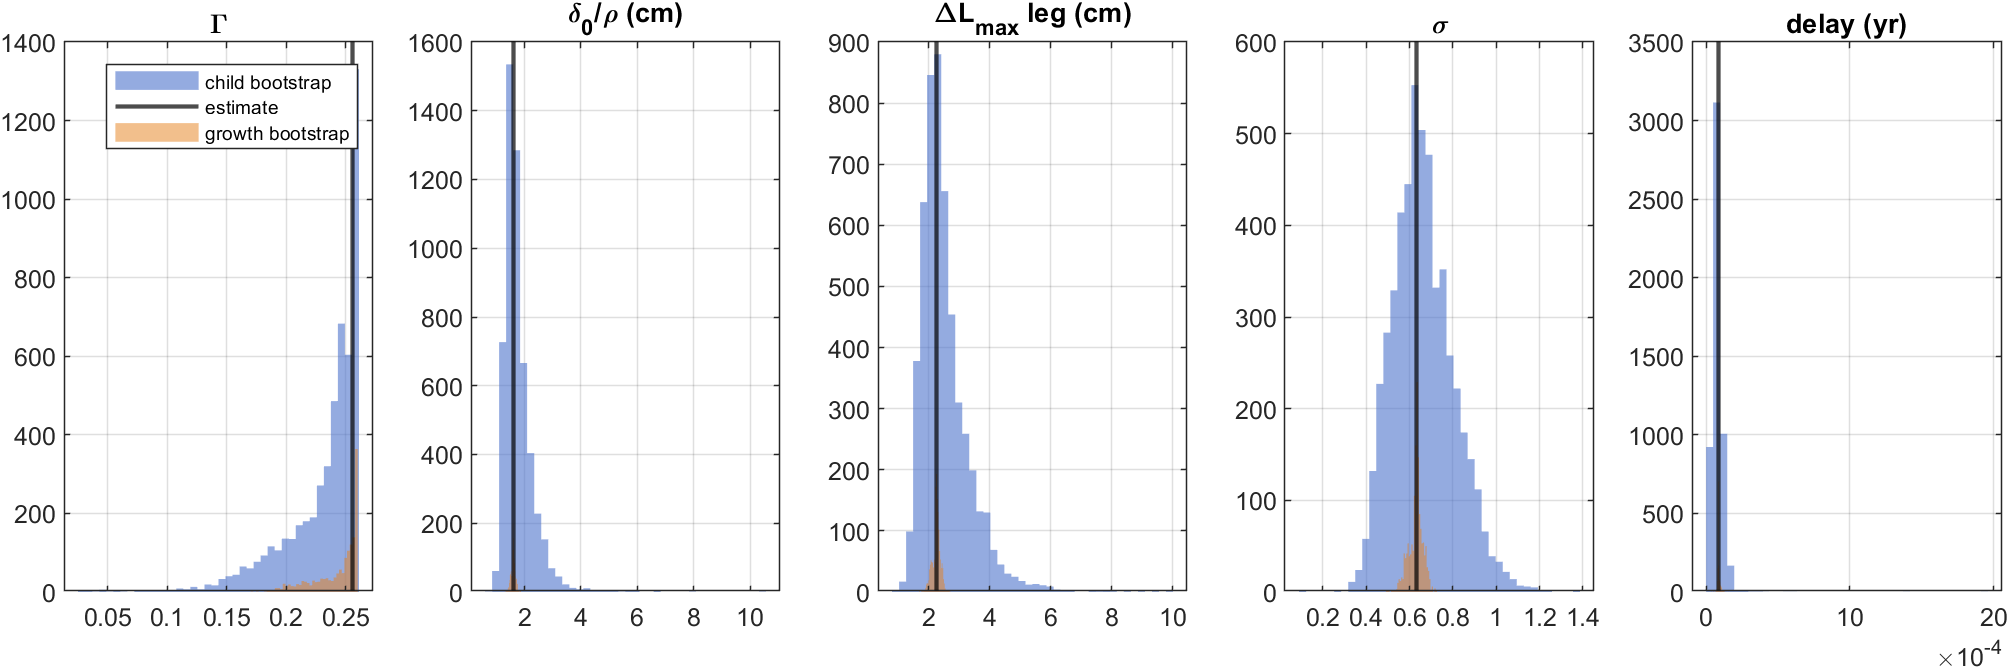
\includegraphics[width=\textwidth]{final_bootstrap_constants.png}
\caption{Distributions of the leg constants over 5,250 child-level bootstrap refits (blue) and 1,500 growth-curve bootstrap refits (orange); black line: estimate. The delay axis is in units of $10^{-4}$ years.}
\label{fig:bootconst}
\end{figure}
Table~\ref{tab:final} and Figure~\ref{fig:bootconst} give the final constants. Growth-curve uncertainty is small next to child-to-child sampling. For the median child the two lengths are $1.31$\,cm (clearance) and $1.85$\,cm (length tolerance); both lie within clinical practice \cite{ghidini2025,ghidiniPoster}. The implausible 2.9\,cm length tolerance of the first pass (Section~\ref{sec:cr}) came from the stand-in ages. With real fitting ages it disappears. The delay is essentially zero: children are fitted soon after amputation.

$\Gamma$ is only bounded from below. The bootstrap piles up against the literature ceiling, and the unbounded fit returns the same value (0.255). The tightness criterion almost never fires first, so the data say only that the circumference tolerance is large ($\Gamma\gtrsim0.15$), which is plausible given socks, liners and heating out \cite{ghidini2025}. This uncertainty does not reach the arm prediction (Sobol index of $\Gamma$ is zero, Section~\ref{sec:sobol}).

\subsection{Fit and out-of-sample performance}
\begin{table}[htbp]
\centering\small
\caption{Final performance (4,000 draws per episode). RMSE of the survival curve, its $R^2$, RMSE of the ``tight'' and ``short'' incidence curves, Harrell's C-index \cite{harrell1982}, and the integrated Brier score \cite{graf1999} with its value for the Kaplan--Meier curve given to every episode (null).}
\label{tab:finalmetrics}
\setlength{\tabcolsep}{4pt}
\begin{tabular}{@{}lccccccc@{}}
\toprule
Set & RMSE & $R^2$ & RMSE tight & RMSE short & C-index & IBS & IBS null\\
\midrule
TT, calibration (188 episodes) & \textbf{0.0150} & \textbf{0.997} & 0.014 & 0.008 & 0.58 & 0.187 & 0.177\\
TT, leave-one-child-out & \textbf{0.0152} & \textbf{0.997} & 0.014 & 0.009 & 0.57 & 0.190 & 0.177\\
KD+TF, held out (85 episodes) & \textbf{0.0228} & \textbf{0.992} & 0.143 & 0.131 & 0.64 & 0.160 & 0.166\\
Noise floor, child bootstrap (median) & 0.033 & -- & 0.030 & 0.024 & -- & -- & --\\
\bottomrule
\end{tabular}
\end{table}

\begin{figure}[htbp]
\centering
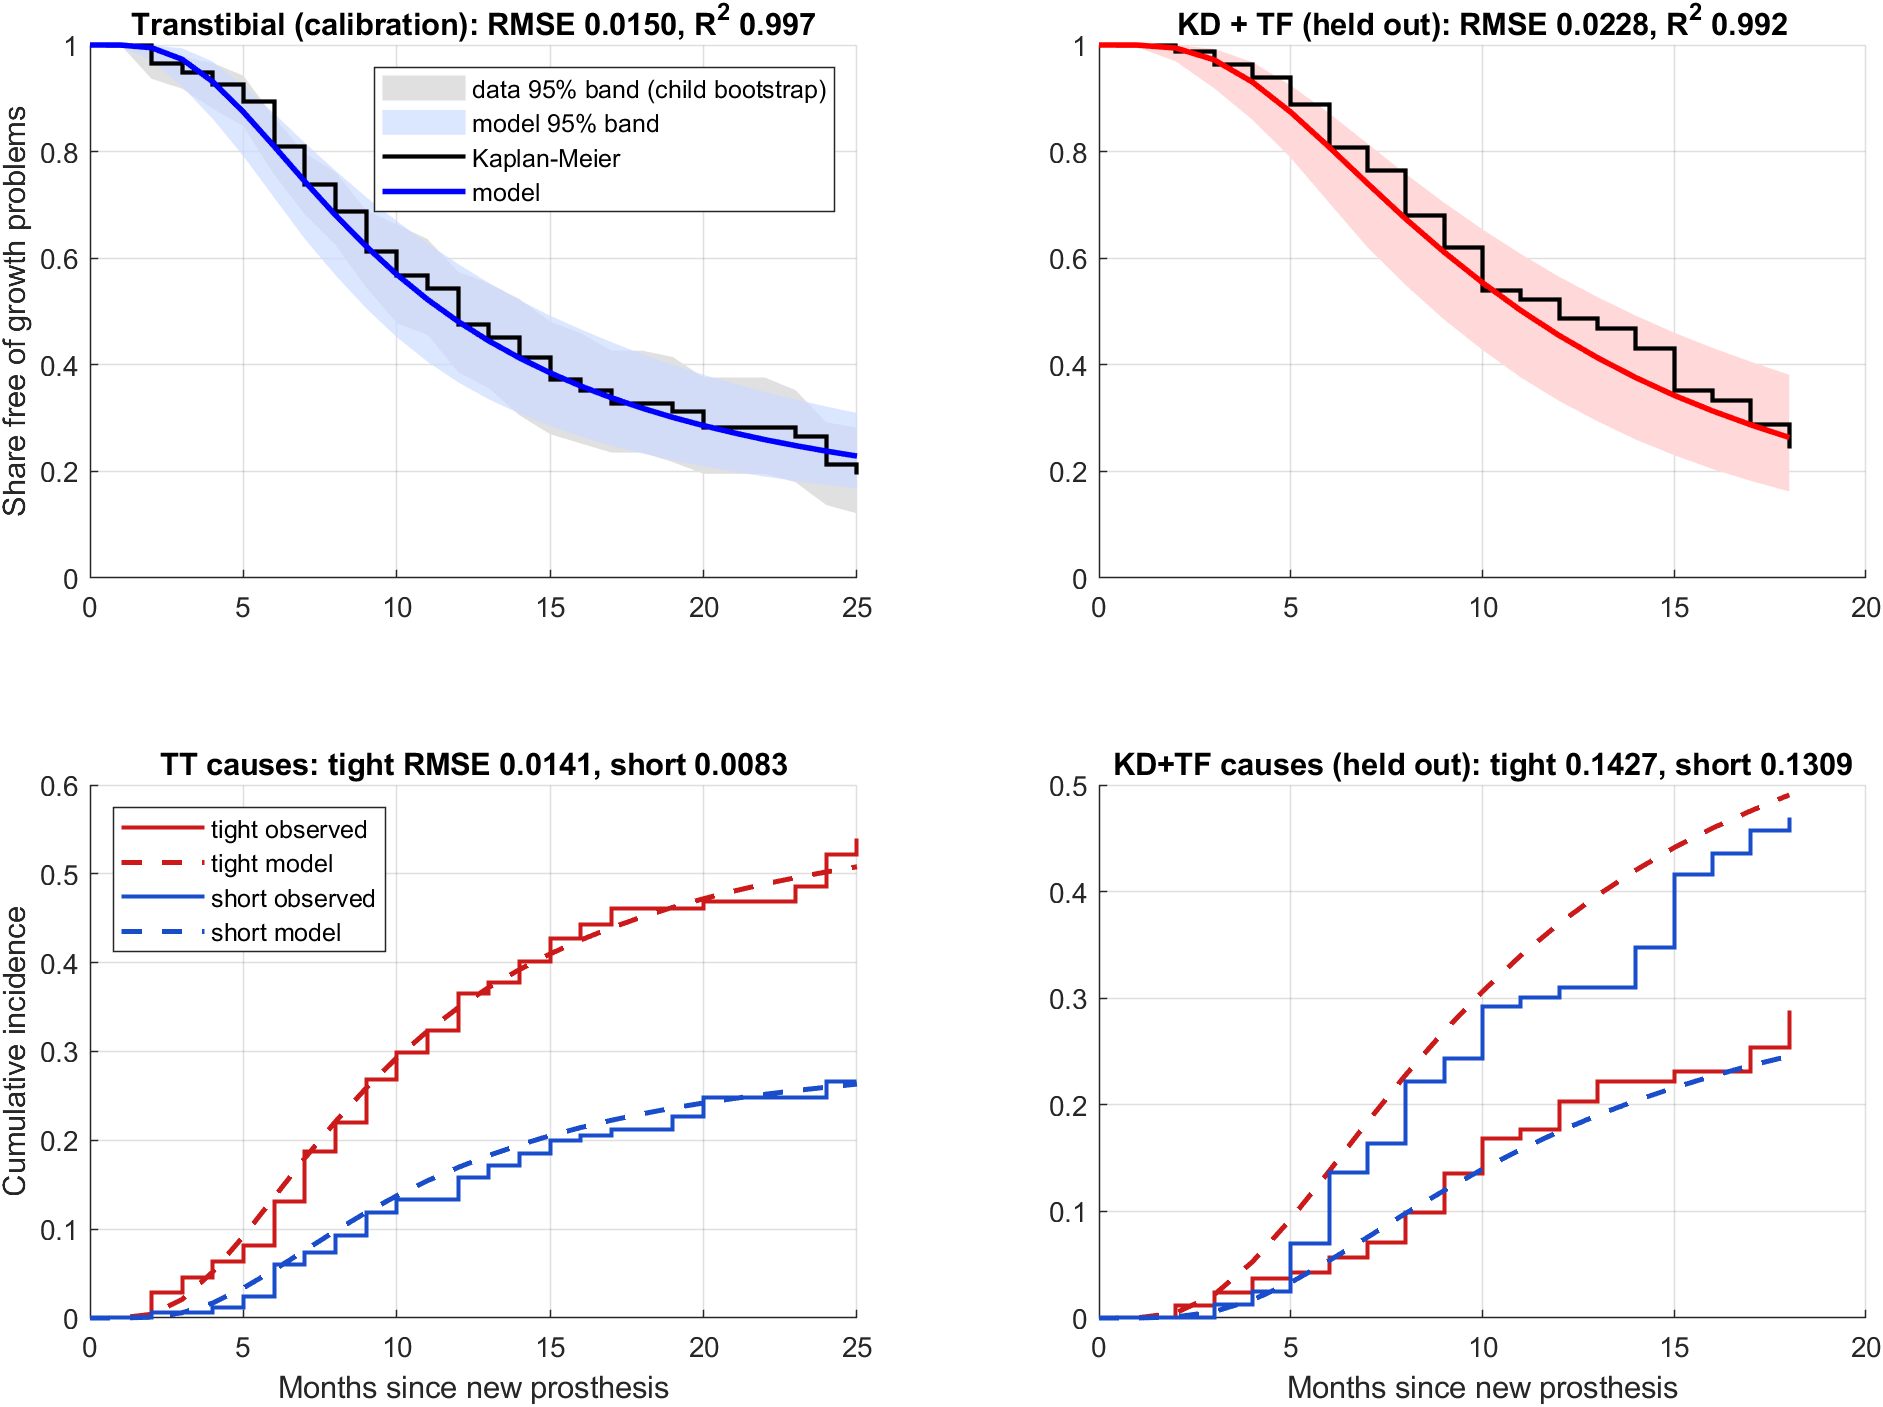
\includegraphics[width=\textwidth]{final_fit.png}
\caption{Final fit. Top: share of sockets free of growth problems, with the 95\% child-bootstrap bands of the data (grey) and of the model (blue). Bottom: cumulative incidence of tight and short problems. Left: transtibial calibration; right: held-out knee-disarticulation and transfemoral episodes.}
\label{fig:finalfit}
\end{figure}

\begin{itemize}[leftmargin=1.4em,itemsep=2pt]
\item \textbf{Population level: excellent.} The survival curve (Figure~\ref{fig:finalfit}) is reproduced with RMSE 0.015 ($R^2=0.997$), and both cause curves to within 0.014. Leaving each child out in turn and predicting that child's sockets gives the same RMSE (0.0152), so the fit is not overfitted. The held-out amputation levels are predicted with RMSE 0.023 ($R^2=0.992$), better than in the first pass (0.029). All of these lie below the child-level noise floor of 0.033 (95\% range 0.014--0.080).
\item \textbf{Mechanism.} In the transtibial leg, first problems are 65\% distal clearance, 34\% length and 1\% tightness. The casefiles' ``tight'' problems are therefore mostly the residual limb reaching the end of the socket. This matches the prosthetists' report that the distal end is where they heat out the socket most \cite{ghidini2025}. The held-out levels still fail mainly through length, which the leg-calibrated cause split does not reproduce (RMSE 0.13--0.14).
\item \textbf{Individual level: weak.} With per-episode ages the model ranks sockets better than chance (C-index 0.58 in the transtibial set, 0.64 held out), and much better than with the stand-in ages (0.51--0.52, Table~\ref{tab:variants}). Its integrated Brier score is, however, no better than giving every socket the population curve (Brier skill $-0.05$ in the transtibial set, $+0.03$ held out). The model predicts \emph{how a population of sockets fails} far better than \emph{which child} will need intervention first. That depends on unrecorded child-level factors, which the model represents only through $\sigma$.
\end{itemize}

\subsection{Model variants}
\begin{table}[htbp]
\centering\footnotesize
\caption{Model variants, each refitted from multiple starts. RMSE of the survival curve (calibration and held out), stacked RMSE of survival and both cause curves, and C-index.}
\label{tab:variants}
\setlength{\tabcolsep}{4pt}
\begin{tabular}{@{}llccccc@{}}
\toprule
Variant & Change & RMSE TT & RMSE KD+TF & Stacked TT & C TT & C KD+TF\\
\midrule
Primary & -- & 0.0149 & 0.0227 & 0.0120 & 0.58 & 0.64\\
Timing only & fit survival only & 0.0146 & 0.0216 & 0.1405 & 0.58 & 0.64\\
Stand-in ages & first-pass ages & 0.0166 & 0.0223 & 0.0136 & 0.51 & 0.52\\
Known ages only & 125 TT episodes & 0.0178 & 0.0449 & 0.0180 & 0.62 & 0.63\\
Socket-level spread & $\sigma$ per socket & 0.0149 & 0.0215 & 0.0121 & 0.58 & 0.64\\
Two-phase growth & spurt curves & 0.0160 & 0.0332 & 0.0158 & 0.56 & 0.64\\
NHANES circumference & modern calf curve & 0.0152 & 0.0205 & 0.0123 & 0.58 & 0.63\\
Anatomical KD/TF & thigh, whole leg & 0.0158 & 0.1746 & 0.0127 & 0.58 & 0.65\\
No delay & delay $=0$ & 0.0149 & 0.0242 & 0.0129 & 0.58 & 0.63\\
$\Gamma$ unbounded & $\Gamma\le0.5$ & 0.0149 & 0.0228 & 0.0122 & 0.58 & 0.64\\
\bottomrule
\end{tabular}
\end{table}
Table~\ref{tab:variants} shows that the conclusions are robust. Modern NHANES growth data, a per-socket spread and an unbounded $\Gamma$ change nothing material. Fitting the survival curve alone matches timing equally well but gets the causes wrong (stacked RMSE 0.14), which is why the causes are fitted. Per-episode ages are what give the model its ranking ability (C 0.58--0.64 against 0.51--0.52). Two variants are instructive failures:
\begin{itemize}[leftmargin=1.4em,itemsep=1pt]
\item \textbf{Anatomical thigh and whole-leg curves for KD and TF} predict the held-out levels far too early (RMSE 0.17). Above-knee sockets evidently tolerate more absolute growth than below-knee ones, plausibly because their length is adjusted more often at the knee unit and pylon.
\item \textbf{The two-phase growth curves}, although they fit the anthropometry better, do not improve the clinical fit.
\end{itemize}

\subsection{Final arm prediction}
\label{sec:armfinal}
\begin{figure}[htbp]
\centering
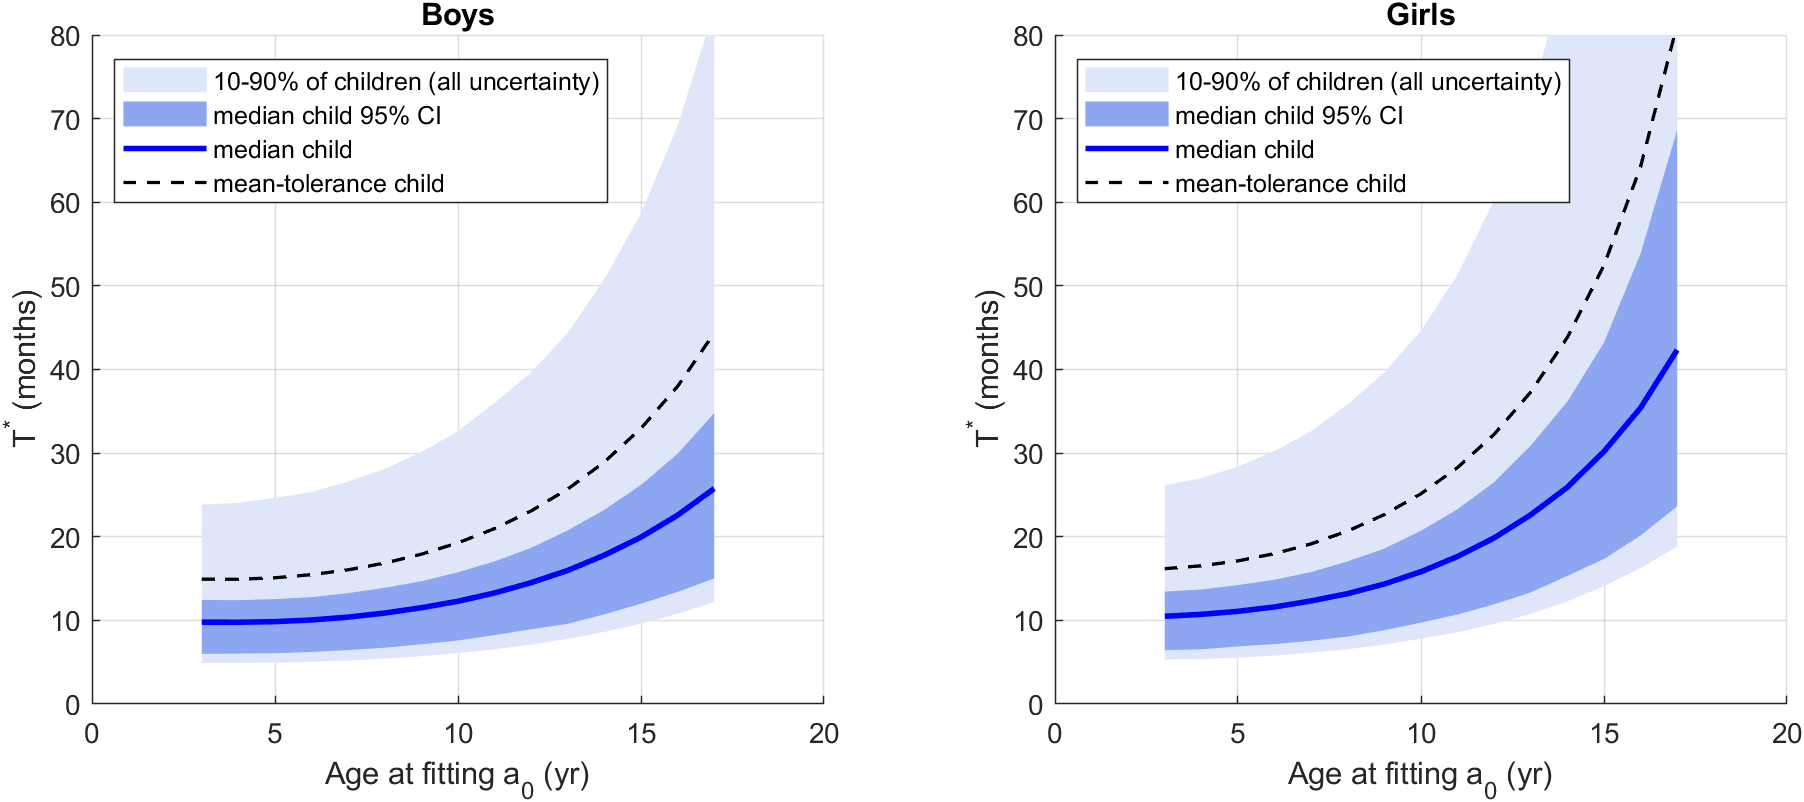
\includegraphics[width=\textwidth]{final_arm_prediction.png}
\caption{Final arm prediction by age at fitting. Line and dark band: median child at central design values, with its 95\% confidence interval from the child and growth bootstraps. Light band: 10--90\% of children when children, constants, growth curves and all design ranges vary together. Dashed: mean-tolerance child (closed form).}
\label{fig:armfinal}
\end{figure}
The final arm prediction (Figure~\ref{fig:armfinal}, Table~\ref{tab:arm}) carries the leg-calibrated, dimensionless constants $\Gamma$ and $\sigma$ (Assumption~\ref{as:transfer}) with their full bootstrap uncertainty, together with the arm growth bootstraps. The median child fitted between 4 and 10 years needs intervention after 9.8--12.3 months (boys) or 10.7--15.8 months (girls). The 95\% confidence interval at age 10 is 7.6--15.8 months for boys and 9.7--20.7 for girls. Allowing for every uncertainty, 80\% of boys fitted at 10 need intervention between 6 and 33 months. No upper-limb casefiles exist to test this directly, but the prediction agrees with clinical guidance for children with upper-limb deficiency, which states that the prosthetic fit of the growing limb must be revised annually \cite{atlas34}: our median child fitted between 4 and 10 years needs intervention after 10--16 months. This is a plausibility check against practice, not a validation.

\subsection{From prediction to practice: a check-up schedule}
\label{sec:schedule}
The arm prediction can be turned into a schedule for a clinic. If the first review after fitting is set at the 25th percentile of the predicted intervals, three children in four are seen before a growth problem develops, without asking families to travel more often than the growth requires. Table~\ref{tab:schedule} gives this time for each fitting age, together with the 10th percentile (the earliest children) and the 50th.

\begin{table}[htbp]
\centering\small
\caption{Recommended first review after fitting a below-elbow socket, in months, from the arm prediction with all uncertainties acting together (children, constants, growth curves and design ranges). At the 25th percentile, 75\% of children are reviewed before a growth problem occurs.}
\label{tab:schedule}
\begin{tabular}{@{}c ccc c ccc@{}}
\toprule
& \multicolumn{3}{c}{Boys} && \multicolumn{3}{c}{Girls}\\
\cmidrule{2-4}\cmidrule{6-8}
Age at fitting & 10\% & \textbf{25\% (review)} & 50\% && 10\% & \textbf{25\% (review)} & 50\%\\
\midrule
4  & 4.9 & \textbf{7.6}  & 11.7 && 5.4 & \textbf{8.3}  & 12.9\\
6  & 5.0 & \textbf{7.8}  & 12.1 && 5.8 & \textbf{9.0}  & 14.1\\
8  & 5.4 & \textbf{8.4}  & 13.2 && 6.6 & \textbf{10.3} & 16.2\\
10 & 6.1 & \textbf{9.5}  & 15.0 && 7.8 & \textbf{12.3} & 19.5\\
12 & 7.1 & \textbf{11.2} & 17.7 && 9.6 & \textbf{15.2} & 24.7\\
\bottomrule
\end{tabular}
\end{table}

\paragraph{Rule of thumb.} Review a child fitted before age 8 about \textbf{8 months} after fitting, and a child fitted at 8--12 after \textbf{9--15 months} (later for girls). Review more often when fitting falls within about two years before the growth spurt: there the two-phase curves shorten the interval by up to 9 months (Section~\ref{sec:spurteffect}). A fixed annual review would see half of the children fitted before age 8 only after their growth problem has begun.

\subsection{Variance-based sensitivity}
\label{sec:sobol}
\begin{figure}[htbp]
\centering
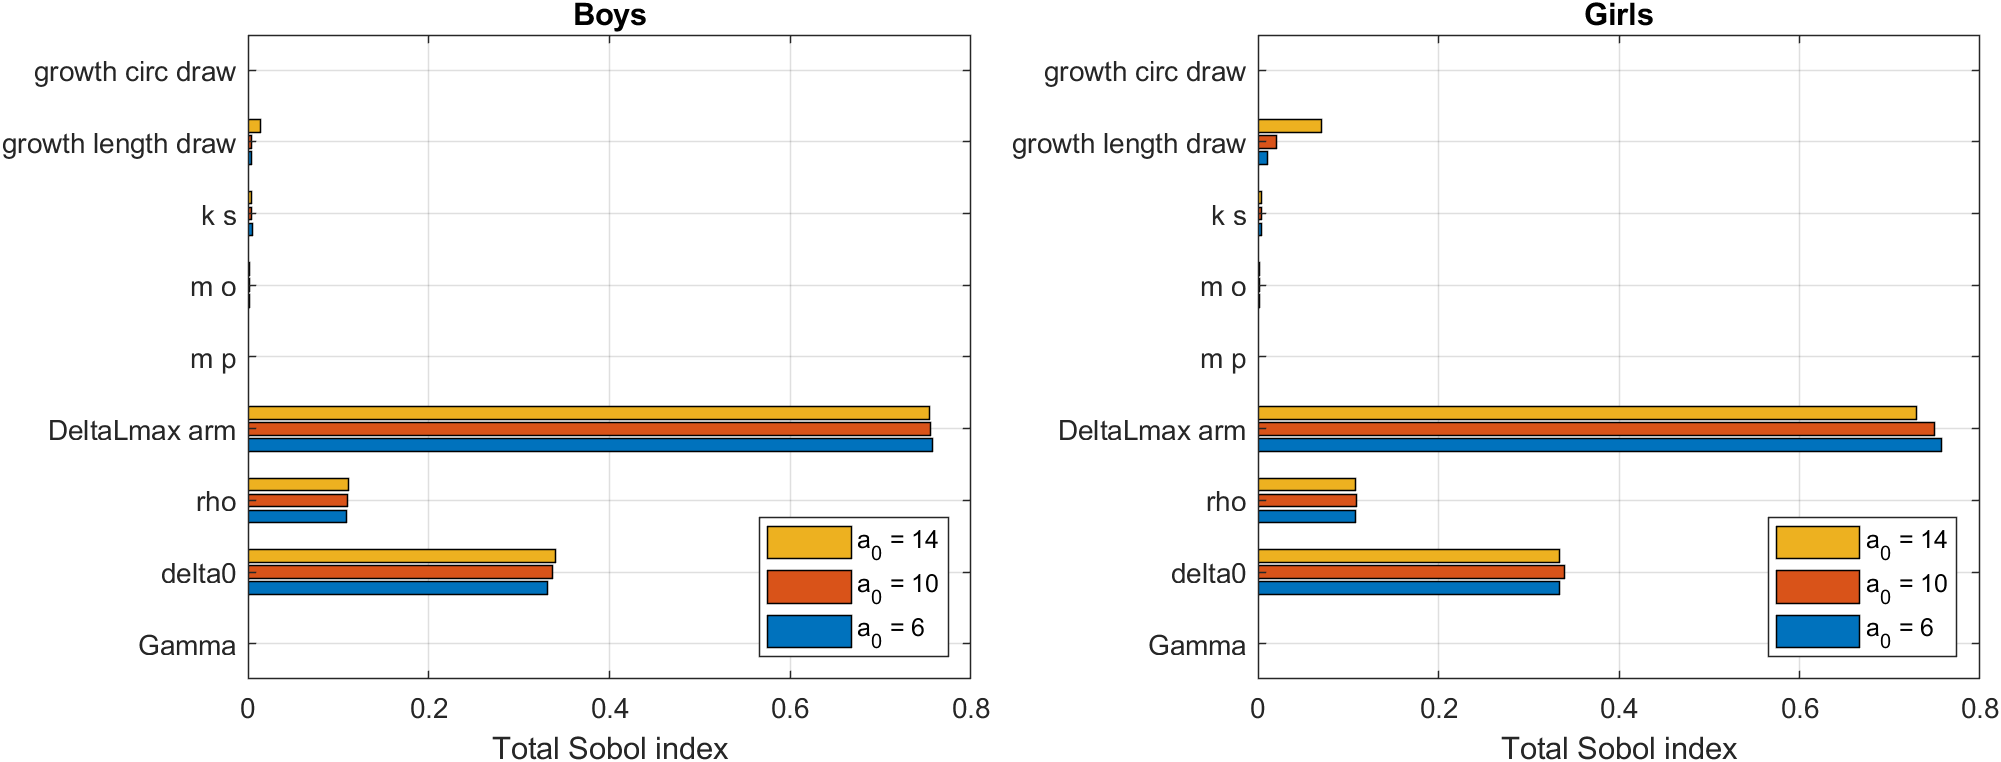
\includegraphics[width=\textwidth]{final_arm_sobol.png}
\caption{Total Sobol indices of the mean-tolerance arm $T^*$ at fitting ages 6, 10 and 14 (131,072 base samples per case, Saltelli--Jansen estimators \cite{saltelli2010}).}
\label{fig:sobol}
\end{figure}
The one-at-a-time analysis of Figure~\ref{fig:tornado} moves one input at a time. Sobol indices \cite{saltelli2010} instead attribute the \emph{variance} of $T^*$ to each input while all inputs vary together over their ranges, interactions included (Figure~\ref{fig:sobol}). The arm length tolerance $\Delta L^{\mathrm{arm}}_{\max}$ explains about 75\% of the variance (total index), the distal clearance $\delta_0$ about 34\% and $\rho$ about 11\%; the indices sum to more than one because these inputs interact through the $\min$ in \eqref{eq:astar}. $\Gamma$, the masses, the liner stiffness and the growth-curve uncertainty each explain less than 2\% (7\% for girls' growth at age 14). The ranking differs from the tornado because over the full box the length criterion often fires before clearance. Both analyses agree on the priority: the arm $\Delta L_{\max}$ and the built-in clearance $\delta_0$ are the two measurements that would sharpen the prediction most.

% =====================================================================
\section{Extension --- compensatory shoulder load}
\label{sec:ext}
% =====================================================================
As a secondary output we add a third action: a straight-arm reach with the upper arm and forearm horizontal ($\varphi=90^\circ$). With the shoulder as pivot, each mass acts at its own lever arm, the upper-arm length $\lua(a)$ plus the fixed forearm arm:
\begin{equation}
\tau_{\mathrm{sh}}(a)=g\big[m_p\big(\lua(a)+\ell_p\big)+m_o\big(\lua(a)+\ell_h\big)\big],
\qquad
S(a)\propto M_b(a)^{2/3},
\qquad
I(a)=\frac{\tau_{\mathrm{sh}}(a)}{M_b(a)^{2/3}} .
\label{eq:shoulder}
\end{equation}
The $2/3$ power is the standard scaling of muscle cross-section, and hence strength, with mass. For boys with the central masses and a prosthesis refitted at each age, $\tau_{\mathrm{sh}}$ rises from 2.43\,N\,m at age 4 to 4.15\,N\,m at 16, but body mass rises faster. The index $I$ therefore \emph{falls}, from 0.360 to 0.251\,N\,m\,kg$^{-2/3}$. With a prosthesis of fixed mass, the youngest children carry the largest relative shoulder load, which supports keeping prostheses for young children as light as possible \cite{frontiers2022}.

% =====================================================================
\section{Strengths, limitations and next steps}
% =====================================================================
\paragraph{Strengths.} Every layer is solved in closed form, so sensitivities are exact and the bands are corner bounds, not samples. All growth constants come from individual records of 3,900 children, with bootstrap uncertainty. The clinical validation uses real per-socket fitting ages, a held-out amputation level and leave-one-child-out prediction. It beats statistical benchmarks and reproduces which problem occurs as well as when. All calibrated constants have 95\% confidence intervals and fall inside independent literature ranges. The edge cases (E1--E7) are handled explicitly.

\paragraph{Drawbacks and how they were addressed.}
\begin{center}
\footnotesize
\renewcommand{\arraystretch}{1.25}
\begin{tabular}{@{}L{5.1cm}L{6.2cm}L{4.4cm}@{}}
\toprule
Drawback & What we did & What remains\\
\midrule
A high $R^2$ on a survival curve can flatter any model & Benchmarked against exponential and Weibull fits; added maximum deviation and band coverage (Section~\ref{sec:bench}) & --\\
The timing fit cannot tell which problem occurs, nor separate clearance from length & Competing-risks fit to the cumulative incidence of tight and short problems (Section~\ref{sec:cr}) & Causes are not transferable between amputation levels\\
The single logistic smooths the pubertal spurt & Two-phase growth curves; effect on $T^*$ quantified and tested on the leg (Sections~\ref{sec:spurt}, \ref{sec:spurteffect}, Table~\ref{tab:variants}) & Two-phase curves do not improve the clinical fit\\
The arm band is wide & Tornado and Sobol analyses rank the inputs: arm $\Delta L_{\max}$, $\delta_0$, then $\rho$ (Sections~\ref{sec:tornado}, \ref{sec:sobol}) & Arm $\delta_0$, $\rho$, $\Delta L_{\max}$ unmeasured\\
One deterministic curve hides differences between children & Median child with 95\% CI and 10--90\% range over children (Table~\ref{tab:arm}) & $\sigma$ is taken from the leg\\
No fitting ages; episodes treated as independent & Raw casefiles re-processed: per-episode ages for 196 episodes, child identifiers, child-level bootstrap and leave-one-child-out validation (Section~\ref{sec:final}) & Ages imputed for children without a recorded age\\
Implausible leg length tolerance (2.9\,cm) & Explained by the stand-in ages; final value 1.85\,cm (median child) & --\\
Growth data are old and from the US & NHANES 1999--2000 cross-check gives the same fit; growth bootstrap shows growth uncertainty is minor & Cambodian growth curves unavailable\\
Constants without uncertainty & 95\% CIs from 5,250 child-level and 1,500 growth-curve bootstrap refits (Table~\ref{tab:final}) & $\Gamma$ only bounded below\\
$R^2=0.9999$ target & Shown to be below the data's noise floor (Section~\ref{sec:r2}) & --\\
\bottomrule
\end{tabular}
\end{center}

\paragraph{Remaining limitations.}
\begin{itemize}[leftmargin=1.4em,itemsep=1pt]
\item The arm prediction rests on leg validation and on agreement with the clinical guideline of annual revision \cite{atlas34}, not on upper-limb outcome data; the arm values of $\delta_0$, $\rho$ and $\Delta L_{\max}$ are unmeasured and set the width of the band.
\item The model predicts populations of sockets far better than individual children: C-index 0.58 (transtibial), 0.64 (held out), and an integrated Brier score no better than the population curve. Which child needs intervention first depends on factors the casefiles do not record.
\item Growth data come from US children in the 1970s; Cambodian children may grow differently. NHANES curves from 1999--2000 give the same fit (Table~\ref{tab:variants}), which suggests the effect is small.
\item The casefiles code distal contact and tightness alike, so the tightness tolerance is only bounded below ($\Gamma\gtrsim0.15$); this does not affect the arm prediction.
\item KD and TF residual limbs are proxied by shank and calf growth. The anatomical thigh mapping predicts them far too early, so above-knee tolerances evidently differ and should be calibrated on their own if more data become available.
\item Statics are quasi-static and planar; dynamic lifting and liner creep are ignored. Masses are held fixed across ages.
\end{itemize}

\paragraph{Next steps.} (i) Measure the length discrepancy children tolerate with an arm prosthesis and the distal clearance built into arm sockets, and obtain the restricted Ghidini growth cohort \cite{ghidiniGrowth} to fix $\rho$; together these explain almost all the variance of the arm prediction (Section~\ref{sec:sobol}). (ii) Validate the two-phase growth curve on the leg casefiles. (iii) Validate on upper-limb casefiles if they become available. (iv) Replace the threshold rule with a stochastic first-passage model, so that child-to-child variation is part of the mechanism rather than calibrated.

% =====================================================================
\section*{Reproducibility}
\addcontentsline{toc}{section}{Reproducibility}
All numbers in this report are produced by scripts in the project folder: \texttt{fit\_growth.py} (first-pass growth fits to the age-group table), \texttt{rmse\_first\_pass/run\_rmse\_calibration.m} (calibration, RMSE, noise floor, held-out test), \texttt{rmse\_first\_pass/sweep\_missing\_constants.m} (sweep of $\rho$ and the flexible model), \texttt{rmse\_first\_pass/address\_drawbacks.m} (competing risks, benchmarks, two-phase growth fits), \texttt{figures/make\_figures.m} (closed-form arm prediction, statics, shoulder index and figures) and \texttt{figures/arm\_sensitivity.m} (tornado, leg-informed scenario, spurt effect). Both use the final growth fits and the final $\Gamma$. Data: \texttt{ghidini\_socket\_episodes.csv}, \texttt{ghidini\_demographics.csv} and \texttt{snyder1977\_growth\_by\_age\_sex.csv}.

The final values (Section~\ref{sec:final}) come from \texttt{final\_study/}:
\begin{itemize}[leftmargin=1.4em,itemsep=1pt]
\item \texttt{scripts/build\_episodes.py} rebuilds the episodes with child identifiers from the raw casefile workbook.
\item \texttt{scripts/tidy\_growth.py} prepares the Snyder individual records and the NHANES files, which \texttt{scripts/ov\_fit\_growth.m} fits (Table~\ref{tab:fits}, Table~\ref{tab:spurt}).
\item \texttt{scripts/overnight\_rmse.m} runs the 3.6-hour study.
\end{itemize}
Every table and figure of that section is written to \texttt{final\_study/results/full/}, with a summary in \texttt{summary.txt}.

% =====================================================================
\begin{thebibliography}{99}
\addcontentsline{toc}{section}{References}
\small
\bibitem{ghidini2025} C.~Ghidini, C.~E.~Edgar, C.~Harte, S.~Kheng, A.~M.~J.~Bull. Impact of physical growth and development on paediatric lower-limb prosthetic provision: prosthetist perspectives and clinical casefile analysis from Cambodia. \emph{Advances in Rehabilitation Science and Practice} 14 (2025). \href{https://doi.org/10.1177/27536351251384354}{doi:10.1177/27536351251384354}.
\bibitem{ghidiniData} C.~Ghidini, C.~E.~Edgar. Data related to 62 clinical casefiles of children with lower limb loss/absence from Cambodia. Zenodo (2024). \href{https://doi.org/10.5281/zenodo.12805856}{doi:10.5281/zenodo.12805856}.
\bibitem{ghidiniGrowth} C.~Ghidini, C.~E.~Edgar, et al. Growth patterns of lower limbs in children with a traumatic transtibial amputation: a retrospective observational cohort study of anthropometric data from Cambodia. \emph{Prosthetics and Orthotics International} (2025). \href{https://doi.org/10.1097/PXR.0000000000000483}{doi:10.1097/PXR.0000000000000483}; data (restricted) \href{https://doi.org/10.5281/zenodo.14187212}{doi:10.5281/zenodo.14187212}.
\bibitem{ghidiniPoster} C.~Ghidini et al. Growth and prosthetic provision in children with below-knee amputation: learnings from low- and high-resource settings. Poster, MSF Scientific Days (2025). \url{https://scienceportal.msf.org/assets/poster-growth-prosthetic-provision-children-below-knee-amputation-learnings-low-resource-high-resource-settings-2025}.
\bibitem{snyder1977} R.~G.~Snyder et al. \emph{Anthropometry of Infants, Children, and Youths to Age 18 for Product Safety Design}. Highway Safety Research Institute, University of Michigan (1977).
\bibitem{anthrokids} NIST AnthroKids: individual-level data of Snyder et al.\ (1977). \url{https://math.nist.gov/~SRessler/anthrokids/}.
\bibitem{luciw2014} M.~D.~Luciw, E.~Jarocka, B.~B.~Edin. Multi-channel EEG recordings during 3,936 grasp and lift trials with varying weight and friction. \emph{Scientific Data} 1 (2014). \href{https://doi.org/10.1038/sdata.2014.47}{doi:10.1038/sdata.2014.47}.
\bibitem{gholizadeh2011} H.~Gholizadeh et al. Photographic measurement of liner--socket pistoning in transtibial prostheses under 30--90\,N static loads. \emph{Prosthetics and Orthotics International} (2011). \href{https://doi.org/10.1177/0309364611423130}{doi:10.1177/0309364611423130}.
\bibitem{atlas34} Upper-limb deficiencies: prosthetic and orthotic management. Chapter 34B in J.~H.~Bowker, J.~W.~Michael (eds.), \emph{Atlas of Limb Prosthetics: Surgical, Prosthetic, and Rehabilitation Principles}, 2nd ed. Mosby-Year Book (1992). Reprinted by the O\&P Virtual Library: \url{https://www.oandplibrary.org/alp/chap34-02.asp}.
\bibitem{sanders2017} J.~E.~Sanders, R.~T.~Youngblood, B.~J.~Hafner, et al. Effects of socket size on metrics of socket fit in trans-tibial prosthesis users. \emph{Medical Engineering \& Physics} 44 (2017) 32--43. \href{https://doi.org/10.1016/j.medengphy.2017.03.003}{doi:10.1016/j.medengphy.2017.03.003}.
\bibitem{volume1} Residual-limb volume changes of about 1\% produce clinically detectable changes in socket fit. PubMed Central PMC7368584. \url{https://pmc.ncbi.nlm.nih.gov/articles/PMC7368584}.
\bibitem{sockply} Bench-top residual-limb model: a 5-ply sock adds about 4\% volume. PubMed Central PMC12614321. \url{https://pmc.ncbi.nlm.nih.gov/articles/PMC12614321/}.
\bibitem{patent} US Patent 11,395,748, Devices, systems, and methods for socket fit management (citing clinically unacceptable fit at about 5\% volume gain).
\bibitem{frontiers2022} Paediatric upper-limb terminal device design (Ottobock Electrohand 2000 for ages 8--13, 130\,g). \emph{Frontiers in Robotics and AI} (2022). \href{https://doi.org/10.3389/frobt.2022.1000159}{doi:10.3389/frobt.2022.1000159}.
\bibitem{dukecase} Case report: below-elbow prosthesis of 240\,g for a child with a very short limb deficiency. DukeSpace, Duke University.
\bibitem{nhanes} Centers for Disease Control and Prevention, National Center for Health Statistics. National Health and Nutrition Examination Survey: body measures and demographics, 1999--2000 and 2017--March 2020. \url{https://wwwn.cdc.gov/nchs/nhanes/}.
\bibitem{imprint} T.~Matray et al. Patient-specific finite element model and experimental interface pressure data for transtibial residuum--socket interaction (IMPRINT). Zenodo (2026). \href{https://doi.org/10.5281/zenodo.23023603}{doi:10.5281/zenodo.23023603}.
\bibitem{harrell1982} F.~E.~Harrell, R.~M.~Califf, D.~B.~Pryor, K.~L.~Lee, R.~A.~Rosati. Evaluating the yield of medical tests. \emph{JAMA} 247 (1982) 2543--2546.
\bibitem{graf1999} E.~Graf, C.~Schmoor, W.~Sauerbrei, M.~Schumacher. Assessment and comparison of prognostic classification schemes for survival data. \emph{Statistics in Medicine} 18 (1999) 2529--2545.
\bibitem{saltelli2010} A.~Saltelli, P.~Annoni, I.~Azzini, F.~Campolongo, M.~Ratto, S.~Tarantola. Variance based sensitivity analysis of model output: design and estimator for the total sensitivity index. \emph{Computer Physics Communications} 181 (2010) 259--270.
\bibitem{otmani2023} S.~Otmani et al. Use of adult anthropometric tables to estimate children body segment inertial parameters. \emph{International Biomechanics} (2023). \href{https://doi.org/10.1080/23335432.2023.2268686}{doi:10.1080/23335432.2023.2268686}.
\end{thebibliography}

\end{document}
